\documentclass[1p]{elsarticle_modified}
%\bibliographystyle{elsarticle-num}

%\usepackage[colorlinks]{hyperref}
%\usepackage{abbrmath_seonhwa} %\Abb, \Ascr, \Acal ,\Abf, \Afrak
\usepackage{amsfonts}
\usepackage{amssymb}
\usepackage{amsmath}
\usepackage{amsthm}
\usepackage{scalefnt}
\usepackage{amsbsy}
\usepackage{kotex}
\usepackage{caption}
\usepackage{subfig}
\usepackage{color}
\usepackage{graphicx}
\usepackage{xcolor} %% white, black, red, green, blue, cyan, magenta, yellow
\usepackage{float}
\usepackage{setspace}
\usepackage{hyperref}

\usepackage{tikz}
\usetikzlibrary{arrows}

\usepackage{multirow}
\usepackage{array} % fixed length table
\usepackage{hhline}

%%%%%%%%%%%%%%%%%%%%%
\makeatletter
\renewcommand*\env@matrix[1][\arraystretch]{%
	\edef\arraystretch{#1}%
	\hskip -\arraycolsep
	\let\@ifnextchar\new@ifnextchar
	\array{*\c@MaxMatrixCols c}}
\makeatother %https://tex.stackexchange.com/questions/14071/how-can-i-increase-the-line-spacing-in-a-matrix
%%%%%%%%%%%%%%%

\usepackage[normalem]{ulem}

\newcommand{\msout}[1]{\ifmmode\text{\sout{\ensuremath{#1}}}\else\sout{#1}\fi}
%SOURCE: \msout is \stkout macro in https://tex.stackexchange.com/questions/20609/strikeout-in-math-mode

\newcommand{\cancel}[1]{
	\ifmmode
	{\color{red}\msout{#1}}
	\else
	{\color{red}\sout{#1}}
	\fi
}

\newcommand{\add}[1]{
	{\color{blue}\uwave{#1}}
}

\newcommand{\replace}[2]{
	\ifmmode
	{\color{red}\msout{#1}}{\color{blue}\uwave{#2}}
	\else
	{\color{red}\sout{#1}}{\color{blue}\uwave{#2}}
	\fi
}

\newcommand{\Sol}{\mathcal{S}} %segment
\newcommand{\D}{D} %diagram
\newcommand{\A}{\mathcal{A}} %arc


%%%%%%%%%%%%%%%%%%%%%%%%%%%%%5 test

\def\sl{\operatorname{\textup{SL}}(2,\Cbb)}
\def\psl{\operatorname{\textup{PSL}}(2,\Cbb)}
\def\quan{\mkern 1mu \triangleright \mkern 1mu}

\theoremstyle{definition}
\newtheorem{thm}{Theorem}[section]
\newtheorem{prop}[thm]{Proposition}
\newtheorem{lem}[thm]{Lemma}
\newtheorem{ques}[thm]{Question}
\newtheorem{cor}[thm]{Corollary}
\newtheorem{defn}[thm]{Definition}
\newtheorem{exam}[thm]{Example}
\newtheorem{rmk}[thm]{Remark}
\newtheorem{alg}[thm]{Algorithm}

\newcommand{\I}{\sqrt{-1}}
\begin{document}

%\begin{frontmatter}
%
%\title{Boundary parabolic representations of knots up to 8 crossings}
%
%%% Group authors per affiliation:
%\author{Yunhi Cho} 
%\address{Department of Mathematics, University of Seoul, Seoul, Korea}
%\ead{yhcho@uos.ac.kr}
%
%
%\author{Seonhwa Kim} %\fnref{s_kim}}
%\address{Center for Geometry and Physics, Institute for Basic Science, Pohang, 37673, Korea}
%\ead{ryeona17@ibs.re.kr}
%
%\author{Hyuk Kim}
%\address{Department of Mathematical Sciences, Seoul National University, Seoul 08826, Korea}
%\ead{hyukkim@snu.ac.kr}
%
%\author{Seokbeom Yoon}
%\address{Department of Mathematical Sciences, Seoul National University, Seoul, 08826,  Korea}
%\ead{sbyoon15@snu.ac.kr}
%
%\begin{abstract}
%We find all boundary parabolic representation of knots up to 8 crossings.
%
%\end{abstract}
%\begin{keyword}
%    \MSC[2010] 57M25 
%\end{keyword}
%
%\end{frontmatter}

%\linenumbers
%\tableofcontents
%
\newcommand\colored[1]{\textcolor{white}{\rule[-0.35ex]{0.8em}{1.4ex}}\kern-0.8em\color{red} #1}%
%\newcommand\colored[1]{\textcolor{white}{ #1}\kern-2.17ex	\textcolor{white}{ #1}\kern-1.81ex	\textcolor{white}{ #1}\kern-2.15ex\color{red}#1	}

{\Large $\underline{12a_{1003}~(K12a_{1003})}$}

\setlength{\tabcolsep}{10pt}
\renewcommand{\arraystretch}{1.6}
\vspace{1cm}\begin{tabular}{m{100pt}>{\centering\arraybackslash}m{274pt}}
\multirow{5}{120pt}{
	\centering
	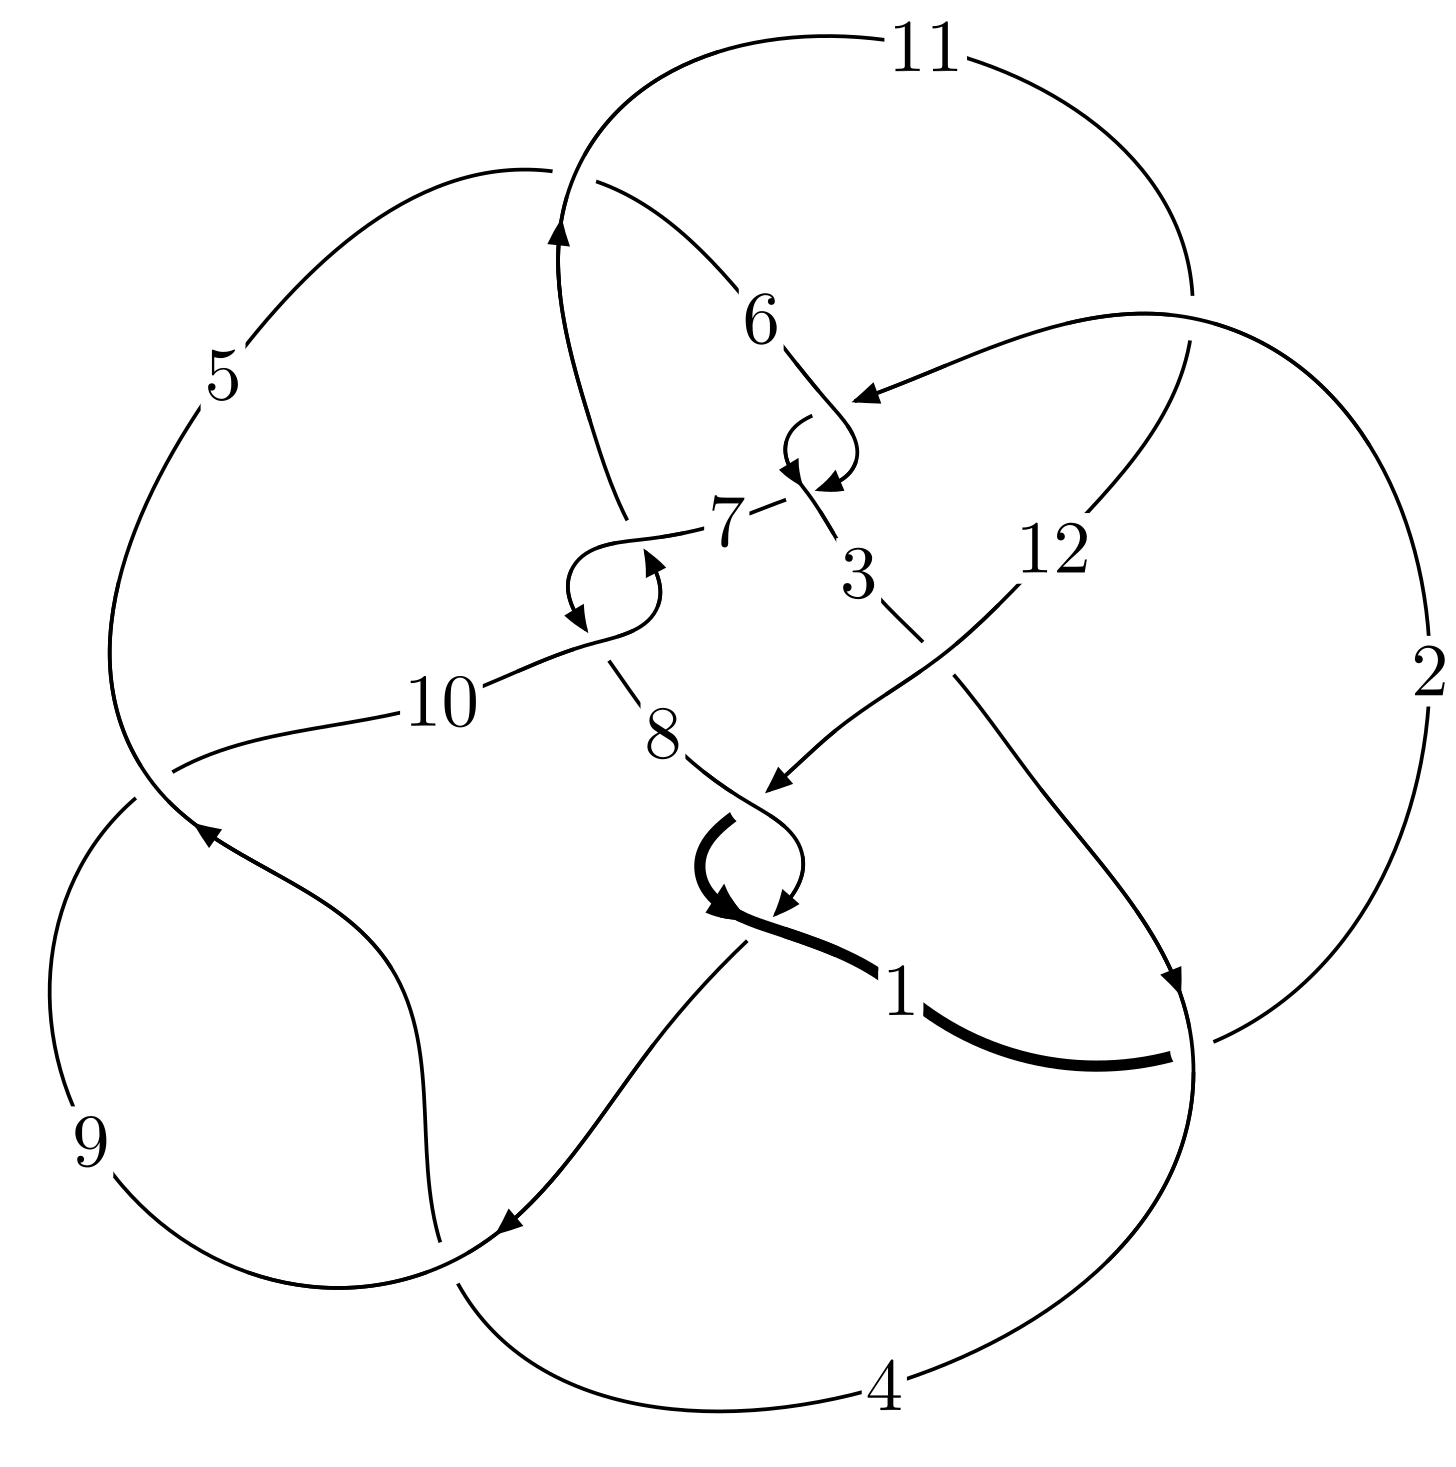
\includegraphics[width=112pt]{../../../GIT/diagram.site/Diagrams/png/1804_12a_1003.png}\\
\ \ \ A knot diagram\footnotemark}&
\allowdisplaybreaks
\textbf{Linearized knot diagam} \\
\cline{2-2}
 &
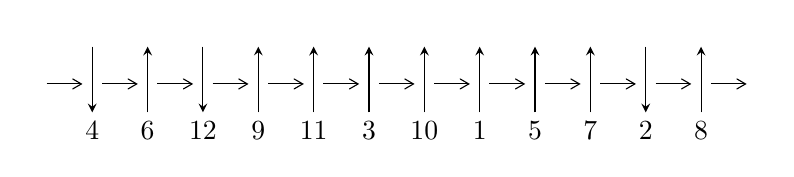
\begin{tikzpicture}[x=20pt, y=17pt]
	% nodes
	\node (C0) at (0, 0) {};
	\node (C1) at (1, 0) {};
	\node (C1U) at (1, +1) {};
	\node (C1D) at (1, -1) {4};

	\node (C2) at (2, 0) {};
	\node (C2U) at (2, +1) {};
	\node (C2D) at (2, -1) {6};

	\node (C3) at (3, 0) {};
	\node (C3U) at (3, +1) {};
	\node (C3D) at (3, -1) {12};

	\node (C4) at (4, 0) {};
	\node (C4U) at (4, +1) {};
	\node (C4D) at (4, -1) {9};

	\node (C5) at (5, 0) {};
	\node (C5U) at (5, +1) {};
	\node (C5D) at (5, -1) {11};

	\node (C6) at (6, 0) {};
	\node (C6U) at (6, +1) {};
	\node (C6D) at (6, -1) {3};

	\node (C7) at (7, 0) {};
	\node (C7U) at (7, +1) {};
	\node (C7D) at (7, -1) {10};

	\node (C8) at (8, 0) {};
	\node (C8U) at (8, +1) {};
	\node (C8D) at (8, -1) {1};

	\node (C9) at (9, 0) {};
	\node (C9U) at (9, +1) {};
	\node (C9D) at (9, -1) {5};

	\node (C10) at (10, 0) {};
	\node (C10U) at (10, +1) {};
	\node (C10D) at (10, -1) {7};

	\node (C11) at (11, 0) {};
	\node (C11U) at (11, +1) {};
	\node (C11D) at (11, -1) {2};

	\node (C12) at (12, 0) {};
	\node (C12U) at (12, +1) {};
	\node (C12D) at (12, -1) {8};
	\node (C13) at (13, 0) {};

	% arrows
	\draw[->,>={angle 60}]
	(C0) edge (C1) (C1) edge (C2) (C2) edge (C3) (C3) edge (C4) (C4) edge (C5) (C5) edge (C6) (C6) edge (C7) (C7) edge (C8) (C8) edge (C9) (C9) edge (C10) (C10) edge (C11) (C11) edge (C12) (C12) edge (C13) ;	\draw[->,>=stealth]
	(C1U) edge (C1D) (C2D) edge (C2U) (C3U) edge (C3D) (C4D) edge (C4U) (C5D) edge (C5U) (C6D) edge (C6U) (C7D) edge (C7U) (C8D) edge (C8U) (C9D) edge (C9U) (C10D) edge (C10U) (C11U) edge (C11D) (C12D) edge (C12U) ;
	\end{tikzpicture} \\
\hhline{~~} \\& 
\textbf{Solving Sequence} \\ \cline{2-2} 
 &
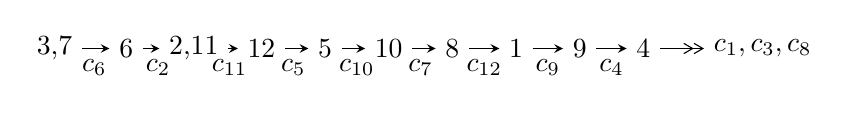
\begin{tikzpicture}[x=23pt, y=7pt]
	% node
	\node (A0) at (-1/8, 0) {3,7};
	\node (A1) at (1, 0) {6};
	\node (A2) at (33/16, 0) {2,11};
	\node (A3) at (25/8, 0) {12};
	\node (A4) at (33/8, 0) {5};
	\node (A5) at (41/8, 0) {10};
	\node (A6) at (49/8, 0) {8};
	\node (A7) at (57/8, 0) {1};
	\node (A8) at (65/8, 0) {9};
	\node (A9) at (73/8, 0) {4};
	\node (C1) at (1/2, -1) {$c_{6}$};
	\node (C2) at (3/2, -1) {$c_{2}$};
	\node (C3) at (21/8, -1) {$c_{11}$};
	\node (C4) at (29/8, -1) {$c_{5}$};
	\node (C5) at (37/8, -1) {$c_{10}$};
	\node (C6) at (45/8, -1) {$c_{7}$};
	\node (C7) at (53/8, -1) {$c_{12}$};
	\node (C8) at (61/8, -1) {$c_{9}$};
	\node (C9) at (69/8, -1) {$c_{4}$};
	\node (A10) at (11, 0) {$c_{1},c_{3},c_{8}$};

	% edge
	\draw[->,>=stealth]	
	(A0) edge (A1) (A1) edge (A2) (A2) edge (A3) (A3) edge (A4) (A4) edge (A5) (A5) edge (A6) (A6) edge (A7) (A7) edge (A8) (A8) edge (A9) ;
	\draw[->>,>={angle 60}]	
	(A9) edge (A10);
\end{tikzpicture} \\ 

\end{tabular} \\

\footnotetext{
The image of knot diagram is generated by the software ``\textbf{Draw programme}" developed by Andrew Bartholomew(\url{http://www.layer8.co.uk/maths/draw/index.htm\#Running-draw}), where we modified some parts for our purpose(\url{https://github.com/CATsTAILs/LinksPainter}).
}\phantom \\ \newline 
\centering \textbf{Ideals for irreducible components\footnotemark of $X_{\text{par}}$} 
 
\begin{align*}
I^u_{1}&=\langle 
3.15863\times10^{750} u^{156}-2.01624\times10^{751} u^{155}+\cdots+4.47851\times10^{751} b-4.21387\times10^{753},\\
\phantom{I^u_{1}}&\phantom{= \langle  }1.25451\times10^{754} u^{156}-7.61396\times10^{754} u^{155}+\cdots+3.94557\times10^{754} a-1.13568\times10^{757},\\
\phantom{I^u_{1}}&\phantom{= \langle  }u^{157}-7 u^{156}+\cdots-3640 u+881\rangle \\
I^u_{2}&=\langle 
-5.77380\times10^{36} u^{40}+1.80943\times10^{37} u^{39}+\cdots+5.47191\times10^{35} b+1.17964\times10^{37},\\
\phantom{I^u_{2}}&\phantom{= \langle  }9.19806\times10^{36} u^{40}-2.98786\times10^{37} u^{39}+\cdots+5.47191\times10^{35} a-2.34136\times10^{37},\;u^{41}-4 u^{40}+\cdots-14 u+1\rangle \\
\\
\end{align*}
\raggedright * 2 irreducible components of $\dim_{\mathbb{C}}=0$, with total 198 representations.\\
\footnotetext{All coefficients of polynomials are rational numbers. But the coefficients are sometimes approximated in decimal forms when there is not enough margin.}
\newpage
\renewcommand{\arraystretch}{1}
\centering \section*{I. $I^u_{1}= \langle 3.16\times10^{750} u^{156}-2.02\times10^{751} u^{155}+\cdots+4.48\times10^{751} b-4.21\times10^{753},\;1.25\times10^{754} u^{156}-7.61\times10^{754} u^{155}+\cdots+3.95\times10^{754} a-1.14\times10^{757},\;u^{157}-7 u^{156}+\cdots-3640 u+881 \rangle$}
\flushleft \textbf{(i) Arc colorings}\\
\begin{tabular}{m{7pt} m{180pt} m{7pt} m{180pt} }
\flushright $a_{3}=$&$\begin{pmatrix}0\\u\end{pmatrix}$ \\
\flushright $a_{7}=$&$\begin{pmatrix}1\\0\end{pmatrix}$ \\
\flushright $a_{6}=$&$\begin{pmatrix}1\\u^2\end{pmatrix}$ \\
\flushright $a_{2}=$&$\begin{pmatrix}- u\\- u^3+u\end{pmatrix}$ \\
\flushright $a_{11}=$&$\begin{pmatrix}-0.317955 u^{156}+1.92975 u^{155}+\cdots-902.978 u+287.837\\-0.0705285 u^{156}+0.450203 u^{155}+\cdots-249.968 u+94.0908\end{pmatrix}$ \\
\flushright $a_{12}=$&$\begin{pmatrix}-0.229475 u^{156}+1.38551 u^{155}+\cdots-632.399 u+196.980\\-0.0987142 u^{156}+0.620635 u^{155}+\cdots-325.032 u+118.759\end{pmatrix}$ \\
\flushright $a_{5}=$&$\begin{pmatrix}-0.501830 u^{156}+3.22052 u^{155}+\cdots-1801.63 u+674.638\\0.244119 u^{156}-1.55615 u^{155}+\cdots+854.846 u-312.508\end{pmatrix}$ \\
\flushright $a_{10}=$&$\begin{pmatrix}-0.247427 u^{156}+1.47955 u^{155}+\cdots-653.011 u+193.746\\-0.0705285 u^{156}+0.450203 u^{155}+\cdots-249.968 u+94.0908\end{pmatrix}$ \\
\flushright $a_{8}=$&$\begin{pmatrix}0.370563 u^{156}-2.33817 u^{155}+\cdots+1251.94 u-440.591\\-0.146125 u^{156}+0.920638 u^{155}+\cdots-493.697 u+177.241\end{pmatrix}$ \\
\flushright $a_{1}=$&$\begin{pmatrix}0.0734131 u^{156}-0.454194 u^{155}+\cdots+248.277 u-72.3291\\-0.125171 u^{156}+0.773007 u^{155}+\cdots-392.350 u+134.951\end{pmatrix}$ \\
\flushright $a_{9}=$&$\begin{pmatrix}0.216606 u^{156}-1.39291 u^{155}+\cdots+853.988 u-318.131\\-0.197723 u^{156}+1.25043 u^{155}+\cdots-704.186 u+256.408\end{pmatrix}$ \\
\flushright $a_{4}=$&$\begin{pmatrix}-0.300574 u^{156}+1.94196 u^{155}+\cdots-1166.78 u+446.927\\0.100662 u^{156}-0.649408 u^{155}+\cdots+395.009 u-145.897\end{pmatrix}$\\&\end{tabular}
\flushleft \textbf{(ii) Obstruction class $= -1$}\\~\\
\flushleft \textbf{(iii) Cusp Shapes $= 0.305069 u^{156}-2.01170 u^{155}+\cdots+1338.49 u-547.708$}\\~\\
\newpage\renewcommand{\arraystretch}{1}
\flushleft \textbf{(iv) u-Polynomials at the component}\newline \\
\begin{tabular}{m{50pt}|m{274pt}}
Crossings & \hspace{64pt}u-Polynomials at each crossing \\
\hline $$\begin{aligned}c_{1}\end{aligned}$$&$\begin{aligned}
&3(3 u^{157}-52 u^{156}+\cdots+6.59843\times10^{9} u-2.50543\times10^{8})
\end{aligned}$\\
\hline $$\begin{aligned}c_{2},c_{6}\end{aligned}$$&$\begin{aligned}
&u^{157}-7 u^{156}+\cdots-3640 u+881
\end{aligned}$\\
\hline $$\begin{aligned}c_{3}\end{aligned}$$&$\begin{aligned}
&u^{157}+4 u^{156}+\cdots-39323 u+2377
\end{aligned}$\\
\hline $$\begin{aligned}c_{4},c_{9}\end{aligned}$$&$\begin{aligned}
&u^{157}+2 u^{156}+\cdots-10946982 u-5026927
\end{aligned}$\\
\hline $$\begin{aligned}c_{5}\end{aligned}$$&$\begin{aligned}
&u^{157}-2 u^{156}+\cdots+20131088 u+6493917
\end{aligned}$\\
\hline $$\begin{aligned}c_{7},c_{10}\end{aligned}$$&$\begin{aligned}
&3(3 u^{157}+u^{156}+\cdots+1673953 u+321907)
\end{aligned}$\\
\hline $$\begin{aligned}c_{8},c_{12}\end{aligned}$$&$\begin{aligned}
&u^{157}+u^{156}+\cdots-122125 u-35417
\end{aligned}$\\
\hline $$\begin{aligned}c_{11}\end{aligned}$$&$\begin{aligned}
&3(3 u^{157}-25 u^{156}+\cdots+1.08396\times10^{7} u-673853)
\end{aligned}$\\
\hline
\end{tabular}\\~\\
\newpage\renewcommand{\arraystretch}{1}
\flushleft \textbf{(v) Riley Polynomials at the component}\newline \\
\begin{tabular}{m{50pt}|m{274pt}}
Crossings & \hspace{64pt}Riley Polynomials at each crossing \\
\hline $$\begin{aligned}c_{1}\end{aligned}$$&$\begin{aligned}
&9(9 y^{157}+458 y^{156}+\cdots+1.96481\times10^{19} y-6.27716\times10^{16})
\end{aligned}$\\
\hline $$\begin{aligned}c_{2},c_{6}\end{aligned}$$&$\begin{aligned}
&y^{157}-87 y^{156}+\cdots+13639002 y-776161
\end{aligned}$\\
\hline $$\begin{aligned}c_{3}\end{aligned}$$&$\begin{aligned}
&y^{157}-4 y^{156}+\cdots-64518507 y-5650129
\end{aligned}$\\
\hline $$\begin{aligned}c_{4},c_{9}\end{aligned}$$&$\begin{aligned}
&y^{157}-126 y^{156}+\cdots+601275991429812 y-25269995063329
\end{aligned}$\\
\hline $$\begin{aligned}c_{5}\end{aligned}$$&$\begin{aligned}
&y^{157}-18 y^{156}+\cdots+2705906604634768 y-42170958002889
\end{aligned}$\\
\hline $$\begin{aligned}c_{7},c_{10}\end{aligned}$$&$\begin{aligned}
&9(9 y^{157}+761 y^{156}+\cdots+9.60988\times10^{11} y-1.03624\times10^{11})
\end{aligned}$\\
\hline $$\begin{aligned}c_{8},c_{12}\end{aligned}$$&$\begin{aligned}
&y^{157}-97 y^{156}+\cdots-7583991957 y-1254363889
\end{aligned}$\\
\hline $$\begin{aligned}c_{11}\end{aligned}$$&$\begin{aligned}
&9(9 y^{157}+359 y^{156}+\cdots+1.54068\times10^{13} y-4.54078\times10^{11})
\end{aligned}$\\
\hline
\end{tabular}\\~\\
\newpage\flushleft \textbf{(vi) Complex Volumes and Cusp Shapes}
$$\begin{array}{c|c|c}  
\text{Solutions to }I^u_{1}& \I (\text{vol} + \sqrt{-1}CS) & \text{Cusp shape}\\
 \hline 
\begin{aligned}
u &= \phantom{-}0.940068 + 0.379267 I \\
a &= -1.98273 - 0.79700 I \\
b &= -0.718037 - 0.916494 I\end{aligned}
 & -0.33928 + 4.05548 I & \phantom{-0.000000 } 0 \\ \hline\begin{aligned}
u &= \phantom{-}0.940068 - 0.379267 I \\
a &= -1.98273 + 0.79700 I \\
b &= -0.718037 + 0.916494 I\end{aligned}
 & -0.33928 - 4.05548 I & \phantom{-0.000000 } 0 \\ \hline\begin{aligned}
u &= -1.002940 + 0.147287 I \\
a &= \phantom{-}0.31203 - 2.13291 I \\
b &= -0.47861 - 2.71346 I\end{aligned}
 & \phantom{-}3.42442 - 0.50214 I & \phantom{-0.000000 } 0 \\ \hline\begin{aligned}
u &= -1.002940 - 0.147287 I \\
a &= \phantom{-}0.31203 + 2.13291 I \\
b &= -0.47861 + 2.71346 I\end{aligned}
 & \phantom{-}3.42442 + 0.50214 I & \phantom{-0.000000 } 0 \\ \hline\begin{aligned}
u &= \phantom{-}0.978634 + 0.274923 I \\
a &= -2.60228 - 0.80680 I \\
b &= -0.273961 - 1.107650 I\end{aligned}
 & -1.97541 + 2.97021 I & \phantom{-0.000000 } 0 \\ \hline\begin{aligned}
u &= \phantom{-}0.978634 - 0.274923 I \\
a &= -2.60228 + 0.80680 I \\
b &= -0.273961 + 1.107650 I\end{aligned}
 & -1.97541 - 2.97021 I & \phantom{-0.000000 } 0 \\ \hline\begin{aligned}
u &= \phantom{-}0.265237 + 0.981962 I \\
a &= -0.240104 - 0.491612 I \\
b &= -0.504910 + 1.246390 I\end{aligned}
 & -0.38275 - 7.61433 I & \phantom{-0.000000 } 0 \\ \hline\begin{aligned}
u &= \phantom{-}0.265237 - 0.981962 I \\
a &= -0.240104 + 0.491612 I \\
b &= -0.504910 - 1.246390 I\end{aligned}
 & -0.38275 + 7.61433 I & \phantom{-0.000000 } 0 \\ \hline\begin{aligned}
u &= -0.211521 + 1.002810 I \\
a &= \phantom{-}0.126460 + 0.448466 I \\
b &= -0.492969 - 1.161370 I\end{aligned}
 & -2.21196 + 2.93997 I & \phantom{-0.000000 } 0 \\ \hline\begin{aligned}
u &= -0.211521 - 1.002810 I \\
a &= \phantom{-}0.126460 - 0.448466 I \\
b &= -0.492969 + 1.161370 I\end{aligned}
 & -2.21196 - 2.93997 I & \phantom{-0.000000 } 0\\
 \hline 
 \end{array}$$\newpage$$\begin{array}{c|c|c}  
\text{Solutions to }I^u_{1}& \I (\text{vol} + \sqrt{-1}CS) & \text{Cusp shape}\\
 \hline 
\begin{aligned}
u &= \phantom{-}0.930229 + 0.430709 I \\
a &= \phantom{-}0.861377 - 0.858328 I \\
b &= \phantom{-}0.301793 + 1.181610 I\end{aligned}
 & \phantom{-}1.63307 + 3.70200 I & \phantom{-0.000000 } 0 \\ \hline\begin{aligned}
u &= \phantom{-}0.930229 - 0.430709 I \\
a &= \phantom{-}0.861377 + 0.858328 I \\
b &= \phantom{-}0.301793 - 1.181610 I\end{aligned}
 & \phantom{-}1.63307 - 3.70200 I & \phantom{-0.000000 } 0 \\ \hline\begin{aligned}
u &= \phantom{-}0.954419 + 0.407482 I \\
a &= \phantom{-}2.25466 + 0.43323 I \\
b &= \phantom{-}0.87448 + 1.23260 I\end{aligned}
 & \phantom{-}3.50050 + 10.88190 I & \phantom{-0.000000 } 0 \\ \hline\begin{aligned}
u &= \phantom{-}0.954419 - 0.407482 I \\
a &= \phantom{-}2.25466 - 0.43323 I \\
b &= \phantom{-}0.87448 - 1.23260 I\end{aligned}
 & \phantom{-}3.50050 - 10.88190 I & \phantom{-0.000000 } 0 \\ \hline\begin{aligned}
u &= \phantom{-}0.936944 + 0.189916 I \\
a &= -1.28703 + 0.78530 I \\
b &= -0.16370 - 1.41273 I\end{aligned}
 & -0.01793 + 4.21639 I & \phantom{-0.000000 } 0 \\ \hline\begin{aligned}
u &= \phantom{-}0.936944 - 0.189916 I \\
a &= -1.28703 - 0.78530 I \\
b &= -0.16370 + 1.41273 I\end{aligned}
 & -0.01793 - 4.21639 I & \phantom{-0.000000 } 0 \\ \hline\begin{aligned}
u &= -0.859317 + 0.409708 I \\
a &= \phantom{-}1.85769 - 0.47809 I \\
b &= \phantom{-}0.349445 - 1.015990 I\end{aligned}
 & -3.38204 - 1.28289 I & \phantom{-0.000000 } 0 \\ \hline\begin{aligned}
u &= -0.859317 - 0.409708 I \\
a &= \phantom{-}1.85769 + 0.47809 I \\
b &= \phantom{-}0.349445 + 1.015990 I\end{aligned}
 & -3.38204 + 1.28289 I & \phantom{-0.000000 } 0 \\ \hline\begin{aligned}
u &= -0.960538 + 0.419471 I \\
a &= -2.17983 - 0.60646 I \\
b &= -0.14648 + 1.45067 I\end{aligned}
 & \phantom{-}0.36542 - 5.39045 I & \phantom{-0.000000 } 0 \\ \hline\begin{aligned}
u &= -0.960538 - 0.419471 I \\
a &= -2.17983 + 0.60646 I \\
b &= -0.14648 - 1.45067 I\end{aligned}
 & \phantom{-}0.36542 + 5.39045 I & \phantom{-0.000000 } 0\\
 \hline 
 \end{array}$$\newpage$$\begin{array}{c|c|c}  
\text{Solutions to }I^u_{1}& \I (\text{vol} + \sqrt{-1}CS) & \text{Cusp shape}\\
 \hline 
\begin{aligned}
u &= -0.992190 + 0.354514 I \\
a &= \phantom{-}2.28833 - 1.24116 I \\
b &= -0.047051 - 0.824743 I\end{aligned}
 & -0.018463 - 1.000730 I & \phantom{-0.000000 } 0 \\ \hline\begin{aligned}
u &= -0.992190 - 0.354514 I \\
a &= \phantom{-}2.28833 + 1.24116 I \\
b &= -0.047051 + 0.824743 I\end{aligned}
 & -0.018463 + 1.000730 I & \phantom{-0.000000 } 0 \\ \hline\begin{aligned}
u &= -0.926433 + 0.168451 I \\
a &= -0.57961 + 1.98870 I \\
b &= \phantom{-}0.41787 + 2.35059 I\end{aligned}
 & \phantom{-}3.26391 - 0.62070 I & \phantom{-0.000000 } 0 \\ \hline\begin{aligned}
u &= -0.926433 - 0.168451 I \\
a &= -0.57961 - 1.98870 I \\
b &= \phantom{-}0.41787 - 2.35059 I\end{aligned}
 & \phantom{-}3.26391 + 0.62070 I & \phantom{-0.000000 } 0 \\ \hline\begin{aligned}
u &= -0.980262 + 0.428091 I \\
a &= -1.80985 + 0.31282 I \\
b &= -0.495296 + 1.319170 I\end{aligned}
 & -1.48693 - 6.48155 I & \phantom{-0.000000 } 0 \\ \hline\begin{aligned}
u &= -0.980262 - 0.428091 I \\
a &= -1.80985 - 0.31282 I \\
b &= -0.495296 - 1.319170 I\end{aligned}
 & -1.48693 + 6.48155 I & \phantom{-0.000000 } 0 \\ \hline\begin{aligned}
u &= \phantom{-}0.315999 + 0.874305 I \\
a &= \phantom{-}0.104004 + 0.663777 I \\
b &= -0.142592 - 1.028540 I\end{aligned}
 & -2.03809 + 2.27481 I & \phantom{-0.000000 } 0 \\ \hline\begin{aligned}
u &= \phantom{-}0.315999 - 0.874305 I \\
a &= \phantom{-}0.104004 - 0.663777 I \\
b &= -0.142592 + 1.028540 I\end{aligned}
 & -2.03809 - 2.27481 I & \phantom{-0.000000 } 0 \\ \hline\begin{aligned}
u &= -0.892387 + 0.605370 I \\
a &= -1.32596 - 1.08784 I \\
b &= -0.026964 + 0.698522 I\end{aligned}
 & \phantom{-}7.95098 + 0.39175 I & \phantom{-0.000000 } 0 \\ \hline\begin{aligned}
u &= -0.892387 - 0.605370 I \\
a &= -1.32596 + 1.08784 I \\
b &= -0.026964 - 0.698522 I\end{aligned}
 & \phantom{-}7.95098 - 0.39175 I & \phantom{-0.000000 } 0\\
 \hline 
 \end{array}$$\newpage$$\begin{array}{c|c|c}  
\text{Solutions to }I^u_{1}& \I (\text{vol} + \sqrt{-1}CS) & \text{Cusp shape}\\
 \hline 
\begin{aligned}
u &= \phantom{-}0.991081 + 0.435230 I \\
a &= \phantom{-}1.83298 + 0.02853 I \\
b &= \phantom{-}0.065159 + 0.986675 I\end{aligned}
 & \phantom{-}0.06925 + 2.18252 I & \phantom{-0.000000 } 0 \\ \hline\begin{aligned}
u &= \phantom{-}0.991081 - 0.435230 I \\
a &= \phantom{-}1.83298 - 0.02853 I \\
b &= \phantom{-}0.065159 - 0.986675 I\end{aligned}
 & \phantom{-}0.06925 - 2.18252 I & \phantom{-0.000000 } 0 \\ \hline\begin{aligned}
u &= -0.886814 + 0.221578 I \\
a &= \phantom{-}0.12838 + 1.89687 I \\
b &= \phantom{-}0.209064 - 1.216420 I\end{aligned}
 & \phantom{-}4.12367 - 9.20788 I & \phantom{-0.000000 } 0 \\ \hline\begin{aligned}
u &= -0.886814 - 0.221578 I \\
a &= \phantom{-}0.12838 - 1.89687 I \\
b &= \phantom{-}0.209064 + 1.216420 I\end{aligned}
 & \phantom{-}4.12367 + 9.20788 I & \phantom{-0.000000 } 0 \\ \hline\begin{aligned}
u &= -0.099493 + 0.902011 I \\
a &= -0.112461 - 0.621935 I \\
b &= \phantom{-}1.007580 + 0.245193 I\end{aligned}
 & \phantom{-}6.76073 - 7.93427 I & \phantom{-0.000000 } 0 \\ \hline\begin{aligned}
u &= -0.099493 - 0.902011 I \\
a &= -0.112461 + 0.621935 I \\
b &= \phantom{-}1.007580 - 0.245193 I\end{aligned}
 & \phantom{-}6.76073 + 7.93427 I & \phantom{-0.000000 } 0 \\ \hline\begin{aligned}
u &= \phantom{-}0.145222 + 0.883203 I \\
a &= -0.054889 - 0.346944 I \\
b &= -0.480987 - 0.231183 I\end{aligned}
 & \phantom{-}1.84082 + 3.69658 I & \phantom{-0.000000 } 0 \\ \hline\begin{aligned}
u &= \phantom{-}0.145222 - 0.883203 I \\
a &= -0.054889 + 0.346944 I \\
b &= -0.480987 + 0.231183 I\end{aligned}
 & \phantom{-}1.84082 - 3.69658 I & \phantom{-0.000000 } 0 \\ \hline\begin{aligned}
u &= \phantom{-}1.084780 + 0.276644 I \\
a &= \phantom{-}1.45784 - 0.01347 I \\
b &= \phantom{-}1.38168 + 0.42360 I\end{aligned}
 & \phantom{-}6.32272 - 0.59511 I & \phantom{-0.000000 } 0 \\ \hline\begin{aligned}
u &= \phantom{-}1.084780 - 0.276644 I \\
a &= \phantom{-}1.45784 + 0.01347 I \\
b &= \phantom{-}1.38168 - 0.42360 I\end{aligned}
 & \phantom{-}6.32272 + 0.59511 I & \phantom{-0.000000 } 0\\
 \hline 
 \end{array}$$\newpage$$\begin{array}{c|c|c}  
\text{Solutions to }I^u_{1}& \I (\text{vol} + \sqrt{-1}CS) & \text{Cusp shape}\\
 \hline 
\begin{aligned}
u &= -0.832564 + 0.276094 I \\
a &= -2.75557 + 1.24139 I \\
b &= \phantom{-}0.192524 + 0.825234 I\end{aligned}
 & \phantom{-}4.07125 + 6.86786 I & \phantom{-0.000000 } 0 \\ \hline\begin{aligned}
u &= -0.832564 - 0.276094 I \\
a &= -2.75557 - 1.24139 I \\
b &= \phantom{-}0.192524 - 0.825234 I\end{aligned}
 & \phantom{-}4.07125 - 6.86786 I & \phantom{-0.000000 } 0 \\ \hline\begin{aligned}
u &= \phantom{-}0.850835 + 0.208150 I \\
a &= \phantom{-}2.37851 + 0.82111 I \\
b &= \phantom{-}0.019601 + 1.135210 I\end{aligned}
 & -0.23173 - 2.34391 I & \phantom{-0.000000 } 0 \\ \hline\begin{aligned}
u &= \phantom{-}0.850835 - 0.208150 I \\
a &= \phantom{-}2.37851 - 0.82111 I \\
b &= \phantom{-}0.019601 - 1.135210 I\end{aligned}
 & -0.23173 + 2.34391 I & \phantom{-0.000000 } 0 \\ \hline\begin{aligned}
u &= \phantom{-}1.12981\phantom{ +0.000000I} \\
a &= -3.99219\phantom{ +0.000000I} \\
b &= -4.88139\phantom{ +0.000000I}\end{aligned}
 & \phantom{-}3.09144\phantom{ +0.000000I} & \phantom{-0.000000 } 0 \\ \hline\begin{aligned}
u &= -0.365591 + 1.071290 I \\
a &= \phantom{-}0.186799 - 0.445736 I \\
b &= \phantom{-}0.227281 + 1.054610 I\end{aligned}
 & -3.89586 + 2.83855 I & \phantom{-0.000000 } 0 \\ \hline\begin{aligned}
u &= -0.365591 - 1.071290 I \\
a &= \phantom{-}0.186799 + 0.445736 I \\
b &= \phantom{-}0.227281 - 1.054610 I\end{aligned}
 & -3.89586 - 2.83855 I & \phantom{-0.000000 } 0 \\ \hline\begin{aligned}
u &= \phantom{-}0.478428 + 1.032730 I \\
a &= \phantom{-}0.435406 - 0.192254 I \\
b &= \phantom{-}0.258703 + 1.148930 I\end{aligned}
 & \phantom{-}3.36390 + 5.17164 I & \phantom{-0.000000 } 0 \\ \hline\begin{aligned}
u &= \phantom{-}0.478428 - 1.032730 I \\
a &= \phantom{-}0.435406 + 0.192254 I \\
b &= \phantom{-}0.258703 - 1.148930 I\end{aligned}
 & \phantom{-}3.36390 - 5.17164 I & \phantom{-0.000000 } 0 \\ \hline\begin{aligned}
u &= -0.237037 + 1.121450 I \\
a &= -0.106545 - 0.177285 I \\
b &= \phantom{-}0.686097 + 1.017130 I\end{aligned}
 & -0.84670 + 4.70707 I & \phantom{-0.000000 } 0\\
 \hline 
 \end{array}$$\newpage$$\begin{array}{c|c|c}  
\text{Solutions to }I^u_{1}& \I (\text{vol} + \sqrt{-1}CS) & \text{Cusp shape}\\
 \hline 
\begin{aligned}
u &= -0.237037 - 1.121450 I \\
a &= -0.106545 + 0.177285 I \\
b &= \phantom{-}0.686097 - 1.017130 I\end{aligned}
 & -0.84670 - 4.70707 I & \phantom{-0.000000 } 0 \\ \hline\begin{aligned}
u &= \phantom{-}1.104340 + 0.348730 I \\
a &= \phantom{-}1.46389 - 0.72900 I \\
b &= \phantom{-}0.937774 - 0.617346 I\end{aligned}
 & \phantom{-}10.37710 + 0.95074 I & \phantom{-0.000000 } 0 \\ \hline\begin{aligned}
u &= \phantom{-}1.104340 - 0.348730 I \\
a &= \phantom{-}1.46389 + 0.72900 I \\
b &= \phantom{-}0.937774 + 0.617346 I\end{aligned}
 & \phantom{-}10.37710 - 0.95074 I & \phantom{-0.000000 } 0 \\ \hline\begin{aligned}
u &= -0.841215\phantom{ +0.000000I} \\
a &= -2.76910\phantom{ +0.000000I} \\
b &= -1.75348\phantom{ +0.000000I}\end{aligned}
 & \phantom{-}2.54729\phantom{ +0.000000I} & \phantom{-0.000000 } 0 \\ \hline\begin{aligned}
u &= -1.136070 + 0.230671 I \\
a &= -1.29900 - 0.66394 I \\
b &= -1.30305 - 0.67519 I\end{aligned}
 & \phantom{-}4.27709 - 0.89813 I & \phantom{-0.000000 } 0 \\ \hline\begin{aligned}
u &= -1.136070 - 0.230671 I \\
a &= -1.29900 + 0.66394 I \\
b &= -1.30305 + 0.67519 I\end{aligned}
 & \phantom{-}4.27709 + 0.89813 I & \phantom{-0.000000 } 0 \\ \hline\begin{aligned}
u &= \phantom{-}0.251700 + 1.132310 I \\
a &= \phantom{-}0.104662 + 0.399000 I \\
b &= \phantom{-}0.605145 - 1.263170 I\end{aligned}
 & \phantom{-}3.5771 - 13.7736 I & \phantom{-0.000000 } 0 \\ \hline\begin{aligned}
u &= \phantom{-}0.251700 - 1.132310 I \\
a &= \phantom{-}0.104662 - 0.399000 I \\
b &= \phantom{-}0.605145 + 1.263170 I\end{aligned}
 & \phantom{-}3.5771 + 13.7736 I & \phantom{-0.000000 } 0 \\ \hline\begin{aligned}
u &= \phantom{-}1.149430 + 0.195951 I \\
a &= \phantom{-}0.767670 - 0.224887 I \\
b &= \phantom{-}0.326737 - 0.396732 I\end{aligned}
 & \phantom{-}2.24833 + 0.22726 I & \phantom{-0.000000 } 0 \\ \hline\begin{aligned}
u &= \phantom{-}1.149430 - 0.195951 I \\
a &= \phantom{-}0.767670 + 0.224887 I \\
b &= \phantom{-}0.326737 + 0.396732 I\end{aligned}
 & \phantom{-}2.24833 - 0.22726 I & \phantom{-0.000000 } 0\\
 \hline 
 \end{array}$$\newpage$$\begin{array}{c|c|c}  
\text{Solutions to }I^u_{1}& \I (\text{vol} + \sqrt{-1}CS) & \text{Cusp shape}\\
 \hline 
\begin{aligned}
u &= \phantom{-}0.672945 + 0.969555 I \\
a &= -0.264643 + 0.570375 I \\
b &= \phantom{-}0.136864 - 1.248680 I\end{aligned}
 & -1.78286 + 2.99407 I & \phantom{-0.000000 } 0 \\ \hline\begin{aligned}
u &= \phantom{-}0.672945 - 0.969555 I \\
a &= -0.264643 - 0.570375 I \\
b &= \phantom{-}0.136864 + 1.248680 I\end{aligned}
 & -1.78286 - 2.99407 I & \phantom{-0.000000 } 0 \\ \hline\begin{aligned}
u &= -0.010867 + 0.811017 I \\
a &= \phantom{-}0.511690 + 0.149434 I \\
b &= \phantom{-}0.432928 - 1.084160 I\end{aligned}
 & \phantom{-}4.97082 - 2.02878 I & \phantom{-0.000000 } 0 \\ \hline\begin{aligned}
u &= -0.010867 - 0.811017 I \\
a &= \phantom{-}0.511690 - 0.149434 I \\
b &= \phantom{-}0.432928 + 1.084160 I\end{aligned}
 & \phantom{-}4.97082 + 2.02878 I & \phantom{-0.000000 } 0 \\ \hline\begin{aligned}
u &= \phantom{-}0.085142 + 0.800877 I \\
a &= -0.243327 + 0.386628 I \\
b &= -0.902161 - 0.085459 I\end{aligned}
 & \phantom{-}3.15585 - 2.56260 I & \phantom{-0.000000 } 0 \\ \hline\begin{aligned}
u &= \phantom{-}0.085142 - 0.800877 I \\
a &= -0.243327 - 0.386628 I \\
b &= -0.902161 + 0.085459 I\end{aligned}
 & \phantom{-}3.15585 + 2.56260 I & \phantom{-0.000000 } 0 \\ \hline\begin{aligned}
u &= -1.004230 + 0.683340 I \\
a &= \phantom{-}0.97985 + 1.09057 I \\
b &= \phantom{-}0.303988 - 0.921871 I\end{aligned}
 & \phantom{-}8.33164 - 5.55456 I & \phantom{-0.000000 } 0 \\ \hline\begin{aligned}
u &= -1.004230 - 0.683340 I \\
a &= \phantom{-}0.97985 - 1.09057 I \\
b &= \phantom{-}0.303988 + 0.921871 I\end{aligned}
 & \phantom{-}8.33164 + 5.55456 I & \phantom{-0.000000 } 0 \\ \hline\begin{aligned}
u &= -1.145370 + 0.409179 I \\
a &= \phantom{-}0.975786 + 0.319146 I \\
b &= \phantom{-}0.683907 + 0.293022 I\end{aligned}
 & \phantom{-}1.48505 - 4.76360 I & \phantom{-0.000000 } 0 \\ \hline\begin{aligned}
u &= -1.145370 - 0.409179 I \\
a &= \phantom{-}0.975786 - 0.319146 I \\
b &= \phantom{-}0.683907 - 0.293022 I\end{aligned}
 & \phantom{-}1.48505 + 4.76360 I & \phantom{-0.000000 } 0\\
 \hline 
 \end{array}$$\newpage$$\begin{array}{c|c|c}  
\text{Solutions to }I^u_{1}& \I (\text{vol} + \sqrt{-1}CS) & \text{Cusp shape}\\
 \hline 
\begin{aligned}
u &= -1.202660 + 0.183165 I \\
a &= \phantom{-}1.61782 + 0.22186 I \\
b &= \phantom{-}0.898146 + 0.290670 I\end{aligned}
 & \phantom{-}11.72880 - 4.15665 I & \phantom{-0.000000 } 0 \\ \hline\begin{aligned}
u &= -1.202660 - 0.183165 I \\
a &= \phantom{-}1.61782 - 0.22186 I \\
b &= \phantom{-}0.898146 - 0.290670 I\end{aligned}
 & \phantom{-}11.72880 + 4.15665 I & \phantom{-0.000000 } 0 \\ \hline\begin{aligned}
u &= \phantom{-}0.588847 + 1.087180 I \\
a &= \phantom{-}0.224007 - 0.403410 I \\
b &= -0.470988 + 0.978656 I\end{aligned}
 & -1.74500 - 0.96923 I & \phantom{-0.000000 } 0 \\ \hline\begin{aligned}
u &= \phantom{-}0.588847 - 1.087180 I \\
a &= \phantom{-}0.224007 + 0.403410 I \\
b &= -0.470988 - 0.978656 I\end{aligned}
 & -1.74500 + 0.96923 I & \phantom{-0.000000 } 0 \\ \hline\begin{aligned}
u &= \phantom{-}0.746225 + 0.148692 I \\
a &= \phantom{-}0.10192 - 1.63298 I \\
b &= -0.112447 + 1.272250 I\end{aligned}
 & -2.96443 - 0.78009 I & \phantom{-0.000000 } 0 \\ \hline\begin{aligned}
u &= \phantom{-}0.746225 - 0.148692 I \\
a &= \phantom{-}0.10192 + 1.63298 I \\
b &= -0.112447 - 1.272250 I\end{aligned}
 & -2.96443 + 0.78009 I & \phantom{-0.000000 } 0 \\ \hline\begin{aligned}
u &= -0.651169 + 0.358375 I \\
a &= \phantom{-}0.0686270 + 0.1063040 I \\
b &= \phantom{-}0.099793 + 1.322930 I\end{aligned}
 & -4.02210 - 2.18252 I & \phantom{-0.000000 } 0 \\ \hline\begin{aligned}
u &= -0.651169 - 0.358375 I \\
a &= \phantom{-}0.0686270 - 0.1063040 I \\
b &= \phantom{-}0.099793 - 1.322930 I\end{aligned}
 & -4.02210 + 2.18252 I & \phantom{-0.000000 } 0 \\ \hline\begin{aligned}
u &= \phantom{-}0.741751\phantom{ +0.000000I} \\
a &= -2.68029\phantom{ +0.000000I} \\
b &= -0.520214\phantom{ +0.000000I}\end{aligned}
 & \phantom{-}0.202774\phantom{ +0.000000I} & \phantom{-0.000000 } 0 \\ \hline\begin{aligned}
u &= \phantom{-}1.230640 + 0.312614 I \\
a &= -0.509647 + 0.563531 I \\
b &= -0.806516 + 0.810081 I\end{aligned}
 & \phantom{-}2.89561 + 0.98168 I & \phantom{-0.000000 } 0\\
 \hline 
 \end{array}$$\newpage$$\begin{array}{c|c|c}  
\text{Solutions to }I^u_{1}& \I (\text{vol} + \sqrt{-1}CS) & \text{Cusp shape}\\
 \hline 
\begin{aligned}
u &= \phantom{-}1.230640 - 0.312614 I \\
a &= -0.509647 - 0.563531 I \\
b &= -0.806516 - 0.810081 I\end{aligned}
 & \phantom{-}2.89561 - 0.98168 I & \phantom{-0.000000 } 0 \\ \hline\begin{aligned}
u &= -1.212490 + 0.378927 I \\
a &= -1.36189 - 0.50506 I \\
b &= -0.936228 + 0.342973 I\end{aligned}
 & \phantom{-}7.09906 - 1.53094 I & \phantom{-0.000000 } 0 \\ \hline\begin{aligned}
u &= -1.212490 - 0.378927 I \\
a &= -1.36189 + 0.50506 I \\
b &= -0.936228 - 0.342973 I\end{aligned}
 & \phantom{-}7.09906 + 1.53094 I & \phantom{-0.000000 } 0 \\ \hline\begin{aligned}
u &= \phantom{-}0.558577 + 0.455748 I \\
a &= \phantom{-}0.179935 - 0.395736 I \\
b &= \phantom{-}0.53765 - 1.34383 I\end{aligned}
 & \phantom{-}2.34201 - 7.23201 I & \phantom{-0.000000 } 0 \\ \hline\begin{aligned}
u &= \phantom{-}0.558577 - 0.455748 I \\
a &= \phantom{-}0.179935 + 0.395736 I \\
b &= \phantom{-}0.53765 + 1.34383 I\end{aligned}
 & \phantom{-}2.34201 + 7.23201 I & \phantom{-0.000000 } 0 \\ \hline\begin{aligned}
u &= \phantom{-}1.192890 + 0.477029 I \\
a &= -1.24954 + 0.68647 I \\
b &= -1.112830 + 0.099371 I\end{aligned}
 & \phantom{-}6.43229 + 7.19422 I & \phantom{-0.000000 } 0 \\ \hline\begin{aligned}
u &= \phantom{-}1.192890 - 0.477029 I \\
a &= -1.24954 - 0.68647 I \\
b &= -1.112830 - 0.099371 I\end{aligned}
 & \phantom{-}6.43229 - 7.19422 I & \phantom{-0.000000 } 0 \\ \hline\begin{aligned}
u &= -1.221780 + 0.411210 I \\
a &= -1.174480 + 0.753815 I \\
b &= -0.038183 + 0.577436 I\end{aligned}
 & \phantom{-}6.83236 - 7.95836 I & \phantom{-0.000000 } 0 \\ \hline\begin{aligned}
u &= -1.221780 - 0.411210 I \\
a &= -1.174480 - 0.753815 I \\
b &= -0.038183 - 0.577436 I\end{aligned}
 & \phantom{-}6.83236 + 7.95836 I & \phantom{-0.000000 } 0 \\ \hline\begin{aligned}
u &= -0.395248 + 0.575371 I \\
a &= \phantom{-}0.470642 + 0.159566 I \\
b &= -0.241293 - 1.308030 I\end{aligned}
 & -3.07407 + 2.55513 I & \phantom{-0.000000 } 0\\
 \hline 
 \end{array}$$\newpage$$\begin{array}{c|c|c}  
\text{Solutions to }I^u_{1}& \I (\text{vol} + \sqrt{-1}CS) & \text{Cusp shape}\\
 \hline 
\begin{aligned}
u &= -0.395248 - 0.575371 I \\
a &= \phantom{-}0.470642 - 0.159566 I \\
b &= -0.241293 + 1.308030 I\end{aligned}
 & -3.07407 - 2.55513 I & \phantom{-0.000000 } 0 \\ \hline\begin{aligned}
u &= -0.303975 + 1.268120 I \\
a &= -0.074618 + 0.413208 I \\
b &= -0.324522 - 1.163040 I\end{aligned}
 & -1.80731 + 6.48795 I & \phantom{-0.000000 } 0 \\ \hline\begin{aligned}
u &= -0.303975 - 1.268120 I \\
a &= -0.074618 - 0.413208 I \\
b &= -0.324522 + 1.163040 I\end{aligned}
 & -1.80731 - 6.48795 I & \phantom{-0.000000 } 0 \\ \hline\begin{aligned}
u &= -1.282640 + 0.235647 I \\
a &= -0.542191 - 0.790232 I \\
b &= -0.572683 - 1.001490 I\end{aligned}
 & \phantom{-}5.05464 + 3.67482 I & \phantom{-0.000000 } 0 \\ \hline\begin{aligned}
u &= -1.282640 - 0.235647 I \\
a &= -0.542191 + 0.790232 I \\
b &= -0.572683 + 1.001490 I\end{aligned}
 & \phantom{-}5.05464 - 3.67482 I & \phantom{-0.000000 } 0 \\ \hline\begin{aligned}
u &= \phantom{-}1.150710 + 0.622498 I \\
a &= \phantom{-}1.365570 - 0.160083 I \\
b &= \phantom{-}0.304017 + 1.166240 I\end{aligned}
 & -0.01137 + 2.86857 I & \phantom{-0.000000 } 0 \\ \hline\begin{aligned}
u &= \phantom{-}1.150710 - 0.622498 I \\
a &= \phantom{-}1.365570 + 0.160083 I \\
b &= \phantom{-}0.304017 - 1.166240 I\end{aligned}
 & -0.01137 - 2.86857 I & \phantom{-0.000000 } 0 \\ \hline\begin{aligned}
u &= \phantom{-}0.652610 + 0.228509 I \\
a &= -1.45929 + 0.45221 I \\
b &= -0.491252 + 1.211040 I\end{aligned}
 & -1.40841 - 1.03482 I & \phantom{-0.000000 } 0 \\ \hline\begin{aligned}
u &= \phantom{-}0.652610 - 0.228509 I \\
a &= -1.45929 - 0.45221 I \\
b &= -0.491252 - 1.211040 I\end{aligned}
 & -1.40841 + 1.03482 I & \phantom{-0.000000 } 0 \\ \hline\begin{aligned}
u &= \phantom{-}1.230150 + 0.457183 I \\
a &= \phantom{-}1.86862 + 0.30880 I \\
b &= \phantom{-}0.595300 + 1.112310 I\end{aligned}
 & \phantom{-}8.63806 + 6.58263 I & \phantom{-0.000000 } 0\\
 \hline 
 \end{array}$$\newpage$$\begin{array}{c|c|c}  
\text{Solutions to }I^u_{1}& \I (\text{vol} + \sqrt{-1}CS) & \text{Cusp shape}\\
 \hline 
\begin{aligned}
u &= \phantom{-}1.230150 - 0.457183 I \\
a &= \phantom{-}1.86862 - 0.30880 I \\
b &= \phantom{-}0.595300 - 1.112310 I\end{aligned}
 & \phantom{-}8.63806 - 6.58263 I & \phantom{-0.000000 } 0 \\ \hline\begin{aligned}
u &= -1.221880 + 0.483922 I \\
a &= \phantom{-}0.118880 + 0.850668 I \\
b &= \phantom{-}0.413748 + 0.836255 I\end{aligned}
 & \phantom{-}8.47557 - 2.60885 I & \phantom{-0.000000 } 0 \\ \hline\begin{aligned}
u &= -1.221880 - 0.483922 I \\
a &= \phantom{-}0.118880 - 0.850668 I \\
b &= \phantom{-}0.413748 - 0.836255 I\end{aligned}
 & \phantom{-}8.47557 + 2.60885 I & \phantom{-0.000000 } 0 \\ \hline\begin{aligned}
u &= -0.002924 + 0.668001 I \\
a &= -0.954122 - 0.485700 I \\
b &= \phantom{-}0.490361 - 0.836450 I\end{aligned}
 & \phantom{-}3.24415 + 3.94333 I & \phantom{-}6.66242 - 2.43245 I \\ \hline\begin{aligned}
u &= -0.002924 - 0.668001 I \\
a &= -0.954122 + 0.485700 I \\
b &= \phantom{-}0.490361 + 0.836450 I\end{aligned}
 & \phantom{-}3.24415 - 3.94333 I & \phantom{-}6.66242 + 2.43245 I \\ \hline\begin{aligned}
u &= \phantom{-}1.335730 + 0.026665 I \\
a &= -0.766227 - 0.149316 I \\
b &= -0.575550 + 0.484274 I\end{aligned}
 & \phantom{-}5.90993 - 1.81141 I & \phantom{-0.000000 } 0 \\ \hline\begin{aligned}
u &= \phantom{-}1.335730 - 0.026665 I \\
a &= -0.766227 + 0.149316 I \\
b &= -0.575550 - 0.484274 I\end{aligned}
 & \phantom{-}5.90993 + 1.81141 I & \phantom{-0.000000 } 0 \\ \hline\begin{aligned}
u &= -1.297560 + 0.347143 I \\
a &= \phantom{-}1.67211 - 0.54276 I \\
b &= \phantom{-}0.498888 - 1.215030 I\end{aligned}
 & \phantom{-}8.77602 - 9.22171 I & \phantom{-0.000000 } 0 \\ \hline\begin{aligned}
u &= -1.297560 - 0.347143 I \\
a &= \phantom{-}1.67211 + 0.54276 I \\
b &= \phantom{-}0.498888 + 1.215030 I\end{aligned}
 & \phantom{-}8.77602 + 9.22171 I & \phantom{-0.000000 } 0 \\ \hline\begin{aligned}
u &= \phantom{-}1.272610 + 0.446499 I \\
a &= \phantom{-}1.29018 - 0.61789 I \\
b &= \phantom{-}1.49289 - 0.13590 I\end{aligned}
 & \phantom{-}10.8950 + 12.6205 I & \phantom{-0.000000 } 0\\
 \hline 
 \end{array}$$\newpage$$\begin{array}{c|c|c}  
\text{Solutions to }I^u_{1}& \I (\text{vol} + \sqrt{-1}CS) & \text{Cusp shape}\\
 \hline 
\begin{aligned}
u &= \phantom{-}1.272610 - 0.446499 I \\
a &= \phantom{-}1.29018 + 0.61789 I \\
b &= \phantom{-}1.49289 + 0.13590 I\end{aligned}
 & \phantom{-}10.8950 - 12.6205 I & \phantom{-0.000000 } 0 \\ \hline\begin{aligned}
u &= -1.276700 + 0.442942 I \\
a &= -1.205910 - 0.120530 I \\
b &= -0.917739 + 0.240078 I\end{aligned}
 & \phantom{-}6.06059 - 8.31394 I & \phantom{-0.000000 } 0 \\ \hline\begin{aligned}
u &= -1.276700 - 0.442942 I \\
a &= -1.205910 + 0.120530 I \\
b &= -0.917739 - 0.240078 I\end{aligned}
 & \phantom{-}6.06059 + 8.31394 I & \phantom{-0.000000 } 0 \\ \hline\begin{aligned}
u &= -1.246350 + 0.566226 I \\
a &= -1.55700 - 0.00197 I \\
b &= -0.67386 + 1.38478 I\end{aligned}
 & \phantom{-}1.02219 - 8.52879 I & \phantom{-0.000000 } 0 \\ \hline\begin{aligned}
u &= -1.246350 - 0.566226 I \\
a &= -1.55700 + 0.00197 I \\
b &= -0.67386 - 1.38478 I\end{aligned}
 & \phantom{-}1.02219 + 8.52879 I & \phantom{-0.000000 } 0 \\ \hline\begin{aligned}
u &= \phantom{-}1.233860 + 0.594092 I \\
a &= -1.76189 + 0.07564 I \\
b &= -0.60762 - 1.33298 I\end{aligned}
 & \phantom{-}2.62811 + 13.31030 I & \phantom{-0.000000 } 0 \\ \hline\begin{aligned}
u &= \phantom{-}1.233860 - 0.594092 I \\
a &= -1.76189 - 0.07564 I \\
b &= -0.60762 + 1.33298 I\end{aligned}
 & \phantom{-}2.62811 - 13.31030 I & \phantom{-0.000000 } 0 \\ \hline\begin{aligned}
u &= -1.240350 + 0.632271 I \\
a &= \phantom{-}1.43435 + 0.05998 I \\
b &= \phantom{-}0.431199 - 1.141240 I\end{aligned}
 & -1.05661 - 8.93991 I & \phantom{-0.000000 } 0 \\ \hline\begin{aligned}
u &= -1.240350 - 0.632271 I \\
a &= \phantom{-}1.43435 - 0.05998 I \\
b &= \phantom{-}0.431199 + 1.141240 I\end{aligned}
 & -1.05661 + 8.93991 I & \phantom{-0.000000 } 0 \\ \hline\begin{aligned}
u &= \phantom{-}0.494053 + 0.335352 I \\
a &= -2.52144 + 0.77520 I \\
b &= \phantom{-}0.358875 - 0.463582 I\end{aligned}
 & \phantom{-}0.494586 - 0.137656 I & \phantom{-}7.45584 - 1.59904 I\\
 \hline 
 \end{array}$$\newpage$$\begin{array}{c|c|c}  
\text{Solutions to }I^u_{1}& \I (\text{vol} + \sqrt{-1}CS) & \text{Cusp shape}\\
 \hline 
\begin{aligned}
u &= \phantom{-}0.494053 - 0.335352 I \\
a &= -2.52144 - 0.77520 I \\
b &= \phantom{-}0.358875 + 0.463582 I\end{aligned}
 & \phantom{-}0.494586 + 0.137656 I & \phantom{-}7.45584 + 1.59904 I \\ \hline\begin{aligned}
u &= \phantom{-}0.385856 + 1.352480 I \\
a &= -0.053478 - 0.324748 I \\
b &= \phantom{-}0.121422 + 0.675308 I\end{aligned}
 & \phantom{-}1.23920 + 4.73510 I & \phantom{-0.000000 } 0 \\ \hline\begin{aligned}
u &= \phantom{-}0.385856 - 1.352480 I \\
a &= -0.053478 + 0.324748 I \\
b &= \phantom{-}0.121422 - 0.675308 I\end{aligned}
 & \phantom{-}1.23920 - 4.73510 I & \phantom{-0.000000 } 0 \\ \hline\begin{aligned}
u &= \phantom{-}1.224880 + 0.697393 I \\
a &= -1.236250 + 0.323383 I \\
b &= -0.599822 - 1.246190 I\end{aligned}
 & \phantom{-}0.49490 + 7.51247 I & \phantom{-0.000000 } 0 \\ \hline\begin{aligned}
u &= \phantom{-}1.224880 - 0.697393 I \\
a &= -1.236250 - 0.323383 I \\
b &= -0.599822 + 1.246190 I\end{aligned}
 & \phantom{-}0.49490 - 7.51247 I & \phantom{-0.000000 } 0 \\ \hline\begin{aligned}
u &= -1.310030 + 0.532093 I \\
a &= \phantom{-}1.105320 + 0.488741 I \\
b &= \phantom{-}0.985273 - 0.830058 I\end{aligned}
 & \phantom{-}10.35490 + 2.57565 I & \phantom{-0.000000 } 0 \\ \hline\begin{aligned}
u &= -1.310030 - 0.532093 I \\
a &= \phantom{-}1.105320 - 0.488741 I \\
b &= \phantom{-}0.985273 + 0.830058 I\end{aligned}
 & \phantom{-}10.35490 - 2.57565 I & \phantom{-0.000000 } 0 \\ \hline\begin{aligned}
u &= -1.27900 + 0.61571 I \\
a &= \phantom{-}1.48471 + 0.10969 I \\
b &= \phantom{-}0.93189 - 1.31791 I\end{aligned}
 & \phantom{-}2.45284 - 10.82650 I & \phantom{-0.000000 } 0 \\ \hline\begin{aligned}
u &= -1.27900 - 0.61571 I \\
a &= \phantom{-}1.48471 - 0.10969 I \\
b &= \phantom{-}0.93189 + 1.31791 I\end{aligned}
 & \phantom{-}2.45284 + 10.82650 I & \phantom{-0.000000 } 0 \\ \hline\begin{aligned}
u &= -0.165472 + 0.550175 I \\
a &= \phantom{-}0.767560 + 0.697747 I \\
b &= \phantom{-}0.216684 + 0.026415 I\end{aligned}
 & -1.35785 + 0.98752 I & -1.29117 - 3.08551 I\\
 \hline 
 \end{array}$$\newpage$$\begin{array}{c|c|c}  
\text{Solutions to }I^u_{1}& \I (\text{vol} + \sqrt{-1}CS) & \text{Cusp shape}\\
 \hline 
\begin{aligned}
u &= -0.165472 - 0.550175 I \\
a &= \phantom{-}0.767560 - 0.697747 I \\
b &= \phantom{-}0.216684 - 0.026415 I\end{aligned}
 & -1.35785 - 0.98752 I & -1.29117 + 3.08551 I \\ \hline\begin{aligned}
u &= -0.545304 + 0.159279 I \\
a &= \phantom{-}1.95040 - 1.87491 I \\
b &= -0.169129 + 1.173590 I\end{aligned}
 & -1.50821 - 1.86231 I & \phantom{-}6.40525 + 3.46383 I \\ \hline\begin{aligned}
u &= -0.545304 - 0.159279 I \\
a &= \phantom{-}1.95040 + 1.87491 I \\
b &= -0.169129 - 1.173590 I\end{aligned}
 & -1.50821 + 1.86231 I & \phantom{-}6.40525 - 3.46383 I \\ \hline\begin{aligned}
u &= \phantom{-}1.29038 + 0.63282 I \\
a &= \phantom{-}1.60527 - 0.08443 I \\
b &= \phantom{-}0.70327 + 1.41141 I\end{aligned}
 & \phantom{-}6.8673 + 20.0217 I & \phantom{-0.000000 } 0 \\ \hline\begin{aligned}
u &= \phantom{-}1.29038 - 0.63282 I \\
a &= \phantom{-}1.60527 + 0.08443 I \\
b &= \phantom{-}0.70327 - 1.41141 I\end{aligned}
 & \phantom{-}6.8673 - 20.0217 I & \phantom{-0.000000 } 0 \\ \hline\begin{aligned}
u &= \phantom{-}1.43902\phantom{ +0.000000I} \\
a &= \phantom{-}0.780025\phantom{ +0.000000I} \\
b &= \phantom{-}1.03725\phantom{ +0.000000I}\end{aligned}
 & \phantom{-}5.83550\phantom{ +0.000000I} & \phantom{-0.000000 } 0 \\ \hline\begin{aligned}
u &= \phantom{-}1.35818 + 0.53888 I \\
a &= -0.523752 + 0.129492 I \\
b &= -0.373814 - 0.226537 I\end{aligned}
 & \phantom{-}5.33089 + 1.99737 I & \phantom{-0.000000 } 0 \\ \hline\begin{aligned}
u &= \phantom{-}1.35818 - 0.53888 I \\
a &= -0.523752 - 0.129492 I \\
b &= -0.373814 + 0.226537 I\end{aligned}
 & \phantom{-}5.33089 - 1.99737 I & \phantom{-0.000000 } 0 \\ \hline\begin{aligned}
u &= -1.31789 + 0.66541 I \\
a &= -1.332690 - 0.031115 I \\
b &= -0.475609 + 1.322890 I\end{aligned}
 & \phantom{-}1.52411 - 13.21170 I & \phantom{-0.000000 } 0 \\ \hline\begin{aligned}
u &= -1.31789 - 0.66541 I \\
a &= -1.332690 + 0.031115 I \\
b &= -0.475609 - 1.322890 I\end{aligned}
 & \phantom{-}1.52411 + 13.21170 I & \phantom{-0.000000 } 0\\
 \hline 
 \end{array}$$\newpage$$\begin{array}{c|c|c}  
\text{Solutions to }I^u_{1}& \I (\text{vol} + \sqrt{-1}CS) & \text{Cusp shape}\\
 \hline 
\begin{aligned}
u &= -1.47475 + 0.19041 I \\
a &= \phantom{-}0.545867 + 0.521383 I \\
b &= \phantom{-}0.732973 + 0.913287 I\end{aligned}
 & \phantom{-}9.88142 + 8.82156 I & \phantom{-0.000000 } 0 \\ \hline\begin{aligned}
u &= -1.47475 - 0.19041 I \\
a &= \phantom{-}0.545867 - 0.521383 I \\
b &= \phantom{-}0.732973 - 0.913287 I\end{aligned}
 & \phantom{-}9.88142 - 8.82156 I & \phantom{-0.000000 } 0 \\ \hline\begin{aligned}
u &= \phantom{-}1.14686 + 0.96038 I \\
a &= -0.605008 + 0.398906 I \\
b &= -0.040711 - 0.781129 I\end{aligned}
 & \phantom{-}5.56411 + 4.17240 I & \phantom{-0.000000 } 0 \\ \hline\begin{aligned}
u &= \phantom{-}1.14686 - 0.96038 I \\
a &= -0.605008 - 0.398906 I \\
b &= -0.040711 + 0.781129 I\end{aligned}
 & \phantom{-}5.56411 - 4.17240 I & \phantom{-0.000000 } 0 \\ \hline\begin{aligned}
u &= \phantom{-}1.43125 + 0.50049 I \\
a &= -0.783624 - 0.155756 I \\
b &= -0.357655 - 0.747380 I\end{aligned}
 & \phantom{-}5.30313 + 2.18170 I & \phantom{-0.000000 } 0 \\ \hline\begin{aligned}
u &= \phantom{-}1.43125 - 0.50049 I \\
a &= -0.783624 + 0.155756 I \\
b &= -0.357655 + 0.747380 I\end{aligned}
 & \phantom{-}5.30313 - 2.18170 I & \phantom{-0.000000 } 0 \\ \hline\begin{aligned}
u &= -0.251646 + 0.406807 I \\
a &= \phantom{-}0.33318 + 2.40544 I \\
b &= -0.299432 - 1.319180 I\end{aligned}
 & -1.29282 + 1.80020 I & \phantom{-}4.94387 - 1.81085 I \\ \hline\begin{aligned}
u &= -0.251646 - 0.406807 I \\
a &= \phantom{-}0.33318 - 2.40544 I \\
b &= -0.299432 + 1.319180 I\end{aligned}
 & -1.29282 - 1.80020 I & \phantom{-}4.94387 + 1.81085 I \\ \hline\begin{aligned}
u &= \phantom{-}0.148503 + 0.430126 I \\
a &= \phantom{-}1.72457 - 0.16017 I \\
b &= \phantom{-}0.757884 + 0.163023 I\end{aligned}
 & \phantom{-}7.69657 + 2.17921 I & \phantom{-}12.55242 - 1.74361 I \\ \hline\begin{aligned}
u &= \phantom{-}0.148503 - 0.430126 I \\
a &= \phantom{-}1.72457 + 0.16017 I \\
b &= \phantom{-}0.757884 - 0.163023 I\end{aligned}
 & \phantom{-}7.69657 - 2.17921 I & \phantom{-}12.55242 + 1.74361 I\\
 \hline 
 \end{array}$$\newpage$$\begin{array}{c|c|c}  
\text{Solutions to }I^u_{1}& \I (\text{vol} + \sqrt{-1}CS) & \text{Cusp shape}\\
 \hline 
\begin{aligned}
u &= \phantom{-}1.51878 + 0.52537 I \\
a &= \phantom{-}0.084289 - 0.175239 I \\
b &= \phantom{-}0.196709 - 0.743397 I\end{aligned}
 & \phantom{-}6.81087 + 2.00402 I & \phantom{-0.000000 } 0 \\ \hline\begin{aligned}
u &= \phantom{-}1.51878 - 0.52537 I \\
a &= \phantom{-}0.084289 + 0.175239 I \\
b &= \phantom{-}0.196709 + 0.743397 I\end{aligned}
 & \phantom{-}6.81087 - 2.00402 I & \phantom{-0.000000 } 0 \\ \hline\begin{aligned}
u &= \phantom{-}1.31809 + 0.95094 I \\
a &= \phantom{-}0.658199 - 0.294699 I \\
b &= \phantom{-}0.224219 + 0.989431 I\end{aligned}
 & \phantom{-}6.01781 + 4.00616 I & \phantom{-0.000000 } 0 \\ \hline\begin{aligned}
u &= \phantom{-}1.31809 - 0.95094 I \\
a &= \phantom{-}0.658199 + 0.294699 I \\
b &= \phantom{-}0.224219 - 0.989431 I\end{aligned}
 & \phantom{-}6.01781 - 4.00616 I & \phantom{-0.000000 } 0 \\ \hline\begin{aligned}
u &= \phantom{-}0.287127\phantom{ +0.000000I} \\
a &= \phantom{-}0.871320\phantom{ +0.000000I} \\
b &= -0.364949\phantom{ +0.000000I}\end{aligned}
 & \phantom{-}0.698705\phantom{ +0.000000I} & \phantom{-}14.8840\phantom{ +0.000000I} \\ \hline\begin{aligned}
u &= -0.079945 + 0.266084 I \\
a &= \phantom{-}1.26621 - 2.63233 I \\
b &= -0.627100 - 0.274595 I\end{aligned}
 & \phantom{-}1.55586 - 0.49268 I & \phantom{-}7.54332 - 0.87240 I \\ \hline\begin{aligned}
u &= -0.079945 - 0.266084 I \\
a &= \phantom{-}1.26621 + 2.63233 I \\
b &= -0.627100 + 0.274595 I\end{aligned}
 & \phantom{-}1.55586 + 0.49268 I & \phantom{-}7.54332 + 0.87240 I\\
 \hline 
 \end{array}$$\newpage\newpage\renewcommand{\arraystretch}{1}
\centering \section*{II. $I^u_{2}= \langle -5.77\times10^{36} u^{40}+1.81\times10^{37} u^{39}+\cdots+5.47\times10^{35} b+1.18\times10^{37},\;9.20\times10^{36} u^{40}-2.99\times10^{37} u^{39}+\cdots+5.47\times10^{35} a-2.34\times10^{37},\;u^{41}-4 u^{40}+\cdots-14 u+1 \rangle$}
\flushleft \textbf{(i) Arc colorings}\\
\begin{tabular}{m{7pt} m{180pt} m{7pt} m{180pt} }
\flushright $a_{3}=$&$\begin{pmatrix}0\\u\end{pmatrix}$ \\
\flushright $a_{7}=$&$\begin{pmatrix}1\\0\end{pmatrix}$ \\
\flushright $a_{6}=$&$\begin{pmatrix}1\\u^2\end{pmatrix}$ \\
\flushright $a_{2}=$&$\begin{pmatrix}- u\\- u^3+u\end{pmatrix}$ \\
\flushright $a_{11}=$&$\begin{pmatrix}-16.8096 u^{40}+54.6037 u^{39}+\cdots-384.073 u+42.7887\\10.5517 u^{40}-33.0677 u^{39}+\cdots+269.069 u-21.5581\end{pmatrix}$ \\
\flushright $a_{12}=$&$\begin{pmatrix}-16.9731 u^{40}+54.5664 u^{39}+\cdots-410.223 u+44.7456\\11.0764 u^{40}-34.7335 u^{39}+\cdots+285.706 u-22.8237\end{pmatrix}$ \\
\flushright $a_{5}=$&$\begin{pmatrix}30.5945 u^{40}-95.7357 u^{39}+\cdots+875.525 u-74.5861\\-8.61959 u^{40}+29.7151 u^{39}+\cdots-163.847 u+13.6794\end{pmatrix}$ \\
\flushright $a_{10}=$&$\begin{pmatrix}-27.3613 u^{40}+87.6713 u^{39}+\cdots-653.141 u+64.3468\\10.5517 u^{40}-33.0677 u^{39}+\cdots+269.069 u-21.5581\end{pmatrix}$ \\
\flushright $a_{8}=$&$\begin{pmatrix}-20.1539 u^{40}+66.6605 u^{39}+\cdots-446.233 u+43.2720\\-0.275367 u^{40}-0.762074 u^{39}+\cdots-37.1858 u+2.13928\end{pmatrix}$ \\
\flushright $a_{1}=$&$\begin{pmatrix}-6.85898 u^{40}+28.4853 u^{39}+\cdots-34.2569 u+15.9890\\-1.93221 u^{40}+8.54124 u^{39}+\cdots+39.0987 u-2.84229\end{pmatrix}$ \\
\flushright $a_{9}=$&$\begin{pmatrix}-47.1489 u^{40}+168.905 u^{39}+\cdots-560.928 u+56.2909\\9.62933 u^{40}-32.9306 u^{39}+\cdots+180.770 u-14.8886\end{pmatrix}$ \\
\flushright $a_{4}=$&$\begin{pmatrix}28.0943 u^{40}-101.022 u^{39}+\cdots+359.949 u-43.5567\\-8.58248 u^{40}+29.6857 u^{39}+\cdots-152.110 u+12.8916\end{pmatrix}$\\&\end{tabular}
\flushleft \textbf{(ii) Obstruction class $= 1$}\\~\\
\flushleft \textbf{(iii) Cusp Shapes $= 78.7593 u^{40}-271.272 u^{39}+\cdots+1093.59 u-89.1575$}\\~\\
\newpage\renewcommand{\arraystretch}{1}
\flushleft \textbf{(iv) u-Polynomials at the component}\newline \\
\begin{tabular}{m{50pt}|m{274pt}}
Crossings & \hspace{64pt}u-Polynomials at each crossing \\
\hline $$\begin{aligned}c_{1}\end{aligned}$$&$\begin{aligned}
&3(3 u^{41}+13 u^{40}+\cdots-13 u+1)
\end{aligned}$\\
\hline $$\begin{aligned}c_{2}\end{aligned}$$&$\begin{aligned}
&u^{41}+4 u^{40}+\cdots-14 u-1
\end{aligned}$\\
\hline $$\begin{aligned}c_{3}\end{aligned}$$&$\begin{aligned}
&u^{41}-3 u^{40}+\cdots+u+1
\end{aligned}$\\
\hline $$\begin{aligned}c_{4}\end{aligned}$$&$\begin{aligned}
&u^{41}+u^{40}+\cdots+4 u+1
\end{aligned}$\\
\hline $$\begin{aligned}c_{5}\end{aligned}$$&$\begin{aligned}
&u^{41}- u^{40}+\cdots-98 u+21
\end{aligned}$\\
\hline $$\begin{aligned}c_{6}\end{aligned}$$&$\begin{aligned}
&u^{41}-4 u^{40}+\cdots-14 u+1
\end{aligned}$\\
\hline $$\begin{aligned}c_{7}\end{aligned}$$&$\begin{aligned}
&3(3 u^{41}+38 u^{40}+\cdots+7 u+1)
\end{aligned}$\\
\hline $$\begin{aligned}c_{8}\end{aligned}$$&$\begin{aligned}
&u^{41}-9 u^{39}+\cdots-19 u-1
\end{aligned}$\\
\hline $$\begin{aligned}c_{9}\end{aligned}$$&$\begin{aligned}
&u^{41}- u^{40}+\cdots+4 u-1
\end{aligned}$\\
\hline $$\begin{aligned}c_{10}\end{aligned}$$&$\begin{aligned}
&3(3 u^{41}-38 u^{40}+\cdots+7 u-1)
\end{aligned}$\\
\hline $$\begin{aligned}c_{11}\end{aligned}$$&$\begin{aligned}
&3(3 u^{41}-26 u^{40}+\cdots-3 u+1)
\end{aligned}$\\
\hline $$\begin{aligned}c_{12}\end{aligned}$$&$\begin{aligned}
&u^{41}-9 u^{39}+\cdots-19 u+1
\end{aligned}$\\
\hline
\end{tabular}\\~\\
\newpage\renewcommand{\arraystretch}{1}
\flushleft \textbf{(v) Riley Polynomials at the component}\newline \\
\begin{tabular}{m{50pt}|m{274pt}}
Crossings & \hspace{64pt}Riley Polynomials at each crossing \\
\hline $$\begin{aligned}c_{1}\end{aligned}$$&$\begin{aligned}
&9(9 y^{41}-343 y^{40}+\cdots+29 y-1)
\end{aligned}$\\
\hline $$\begin{aligned}c_{2},c_{6}\end{aligned}$$&$\begin{aligned}
&y^{41}-20 y^{40}+\cdots+164 y-1
\end{aligned}$\\
\hline $$\begin{aligned}c_{3}\end{aligned}$$&$\begin{aligned}
&y^{41}-9 y^{40}+\cdots+15 y-1
\end{aligned}$\\
\hline $$\begin{aligned}c_{4},c_{9}\end{aligned}$$&$\begin{aligned}
&y^{41}-39 y^{40}+\cdots+14 y-1
\end{aligned}$\\
\hline $$\begin{aligned}c_{5}\end{aligned}$$&$\begin{aligned}
&y^{41}+9 y^{40}+\cdots+14098 y-441
\end{aligned}$\\
\hline $$\begin{aligned}c_{7},c_{10}\end{aligned}$$&$\begin{aligned}
&9(9 y^{41}-112 y^{40}+\cdots-245 y-1)
\end{aligned}$\\
\hline $$\begin{aligned}c_{8},c_{12}\end{aligned}$$&$\begin{aligned}
&y^{41}-18 y^{40}+\cdots+261 y-1
\end{aligned}$\\
\hline $$\begin{aligned}c_{11}\end{aligned}$$&$\begin{aligned}
&9(9 y^{41}-298 y^{40}+\cdots+23 y-1)
\end{aligned}$\\
\hline
\end{tabular}\\~\\
\newpage\flushleft \textbf{(vi) Complex Volumes and Cusp Shapes}
$$\begin{array}{c|c|c}  
\text{Solutions to }I^u_{2}& \I (\text{vol} + \sqrt{-1}CS) & \text{Cusp shape}\\
 \hline 
\begin{aligned}
u &= -0.967192 + 0.276575 I \\
a &= -2.34467 + 1.19064 I \\
b &= -0.513333 + 1.085480 I\end{aligned}
 & -0.05487 - 3.00795 I & \phantom{-}10.53277 + 3.04890 I \\ \hline\begin{aligned}
u &= -0.967192 - 0.276575 I \\
a &= -2.34467 - 1.19064 I \\
b &= -0.513333 - 1.085480 I\end{aligned}
 & -0.05487 + 3.00795 I & \phantom{-}10.53277 - 3.04890 I \\ \hline\begin{aligned}
u &= \phantom{-}0.917296 + 0.374401 I \\
a &= -1.93922 + 0.77186 I \\
b &= -0.235092 - 1.333590 I\end{aligned}
 & -1.07814 + 4.47132 I & \phantom{-}3.31883 - 6.44593 I \\ \hline\begin{aligned}
u &= \phantom{-}0.917296 - 0.374401 I \\
a &= -1.93922 - 0.77186 I \\
b &= -0.235092 + 1.333590 I\end{aligned}
 & -1.07814 - 4.47132 I & \phantom{-}3.31883 + 6.44593 I \\ \hline\begin{aligned}
u &= \phantom{-}0.957227 + 0.369955 I \\
a &= \phantom{-}2.11553 + 0.67760 I \\
b &= \phantom{-}0.047538 + 0.842774 I\end{aligned}
 & -1.28013 + 1.50111 I & \phantom{-}4.03097 - 2.30869 I \\ \hline\begin{aligned}
u &= \phantom{-}0.957227 - 0.369955 I \\
a &= \phantom{-}2.11553 - 0.67760 I \\
b &= \phantom{-}0.047538 - 0.842774 I\end{aligned}
 & -1.28013 - 1.50111 I & \phantom{-}4.03097 + 2.30869 I \\ \hline\begin{aligned}
u &= \phantom{-}0.530210 + 0.810440 I \\
a &= \phantom{-}0.710976 - 0.666761 I \\
b &= -0.315679 + 1.151370 I\end{aligned}
 & -2.42496 - 0.20996 I & \phantom{-}2.55692 - 2.02439 I \\ \hline\begin{aligned}
u &= \phantom{-}0.530210 - 0.810440 I \\
a &= \phantom{-}0.710976 + 0.666761 I \\
b &= -0.315679 - 1.151370 I\end{aligned}
 & -2.42496 + 0.20996 I & \phantom{-}2.55692 + 2.02439 I \\ \hline\begin{aligned}
u &= -0.957972 + 0.430465 I \\
a &= \phantom{-}1.41892 + 1.18660 I \\
b &= \phantom{-}0.646242 - 0.047894 I\end{aligned}
 & \phantom{-}8.98186 + 0.39614 I & \phantom{-}15.1411 + 0. I\phantom{ +0.000000I} \\ \hline\begin{aligned}
u &= -0.957972 - 0.430465 I \\
a &= \phantom{-}1.41892 - 1.18660 I \\
b &= \phantom{-}0.646242 + 0.047894 I\end{aligned}
 & \phantom{-}8.98186 - 0.39614 I & \phantom{-}15.1411 + 0. I\phantom{ +0.000000I}\\
 \hline 
 \end{array}$$\newpage$$\begin{array}{c|c|c}  
\text{Solutions to }I^u_{2}& \I (\text{vol} + \sqrt{-1}CS) & \text{Cusp shape}\\
 \hline 
\begin{aligned}
u &= -1.10437\phantom{ +0.000000I} \\
a &= -5.17172\phantom{ +0.000000I} \\
b &= -6.08818\phantom{ +0.000000I}\end{aligned}
 & \phantom{-}3.11824\phantom{ +0.000000I} & \phantom{-}205.070\phantom{ +0.000000I} \\ \hline\begin{aligned}
u &= \phantom{-}0.886514\phantom{ +0.000000I} \\
a &= -3.03550\phantom{ +0.000000I} \\
b &= -1.93867\phantom{ +0.000000I}\end{aligned}
 & \phantom{-}2.73703\phantom{ +0.000000I} & \phantom{-}29.8820\phantom{ +0.000000I} \\ \hline\begin{aligned}
u &= \phantom{-}0.412391 + 0.751176 I \\
a &= -0.288581 + 1.215010 I \\
b &= -0.051027 - 1.286210 I\end{aligned}
 & -1.61210 + 4.07460 I & \phantom{-}5.53794 - 6.18665 I \\ \hline\begin{aligned}
u &= \phantom{-}0.412391 - 0.751176 I \\
a &= -0.288581 - 1.215010 I \\
b &= -0.051027 + 1.286210 I\end{aligned}
 & -1.61210 - 4.07460 I & \phantom{-}5.53794 + 6.18665 I \\ \hline\begin{aligned}
u &= -1.034310 + 0.494300 I \\
a &= -0.892975 - 0.699136 I \\
b &= -0.0244412 + 0.0814704 I\end{aligned}
 & \phantom{-}9.25914 - 4.28800 I & \phantom{-}14.2709 + 3.4191 I \\ \hline\begin{aligned}
u &= -1.034310 - 0.494300 I \\
a &= -0.892975 + 0.699136 I \\
b &= -0.0244412 - 0.0814704 I\end{aligned}
 & \phantom{-}9.25914 + 4.28800 I & \phantom{-}14.2709 - 3.4191 I \\ \hline\begin{aligned}
u &= -0.286646 + 1.124780 I \\
a &= \phantom{-}0.054480 + 0.327935 I \\
b &= -0.559946 - 1.046810 I\end{aligned}
 & -2.21574 + 3.68999 I & \phantom{-}6.00000 - 8.07545 I \\ \hline\begin{aligned}
u &= -0.286646 - 1.124780 I \\
a &= \phantom{-}0.054480 - 0.327935 I \\
b &= -0.559946 + 1.046810 I\end{aligned}
 & -2.21574 - 3.68999 I & \phantom{-}6.00000 + 8.07545 I \\ \hline\begin{aligned}
u &= -0.800978 + 0.205134 I \\
a &= -1.065430 + 0.712656 I \\
b &= -0.367763 - 1.235220 I\end{aligned}
 & -0.769602 + 0.776118 I & \phantom{-}12.89317 + 1.67571 I \\ \hline\begin{aligned}
u &= -0.800978 - 0.205134 I \\
a &= -1.065430 - 0.712656 I \\
b &= -0.367763 + 1.235220 I\end{aligned}
 & -0.769602 - 0.776118 I & \phantom{-}12.89317 - 1.67571 I\\
 \hline 
 \end{array}$$\newpage$$\begin{array}{c|c|c}  
\text{Solutions to }I^u_{2}& \I (\text{vol} + \sqrt{-1}CS) & \text{Cusp shape}\\
 \hline 
\begin{aligned}
u &= \phantom{-}0.386012 + 0.663461 I \\
a &= \phantom{-}0.444495 + 0.472978 I \\
b &= -0.147129 - 1.096260 I\end{aligned}
 & -2.95452 + 2.14772 I & -0.86553 - 3.38082 I \\ \hline\begin{aligned}
u &= \phantom{-}0.386012 - 0.663461 I \\
a &= \phantom{-}0.444495 - 0.472978 I \\
b &= -0.147129 + 1.096260 I\end{aligned}
 & -2.95452 - 2.14772 I & -0.86553 + 3.38082 I \\ \hline\begin{aligned}
u &= \phantom{-}1.231620 + 0.160871 I \\
a &= -1.124090 + 0.424481 I \\
b &= -1.302950 + 0.441045 I\end{aligned}
 & \phantom{-}4.15697 + 0.17532 I & \phantom{-0.000000 } 0 \\ \hline\begin{aligned}
u &= \phantom{-}1.231620 - 0.160871 I \\
a &= -1.124090 - 0.424481 I \\
b &= -1.302950 - 0.441045 I\end{aligned}
 & \phantom{-}4.15697 - 0.17532 I & \phantom{-0.000000 } 0 \\ \hline\begin{aligned}
u &= -1.266290 + 0.322271 I \\
a &= \phantom{-}1.39309 - 0.89120 I \\
b &= \phantom{-}0.518096 - 0.955301 I\end{aligned}
 & \phantom{-}6.90593 - 9.52644 I & \phantom{-0.000000 } 0 \\ \hline\begin{aligned}
u &= -1.266290 - 0.322271 I \\
a &= \phantom{-}1.39309 + 0.89120 I \\
b &= \phantom{-}0.518096 + 0.955301 I\end{aligned}
 & \phantom{-}6.90593 + 9.52644 I & \phantom{-0.000000 } 0 \\ \hline\begin{aligned}
u &= \phantom{-}0.279885 + 1.313700 I \\
a &= \phantom{-}0.066965 - 0.177930 I \\
b &= \phantom{-}0.252183 + 0.794730 I\end{aligned}
 & \phantom{-}1.00126 + 5.06650 I & \phantom{-0.000000 } 0 \\ \hline\begin{aligned}
u &= \phantom{-}0.279885 - 1.313700 I \\
a &= \phantom{-}0.066965 + 0.177930 I \\
b &= \phantom{-}0.252183 - 0.794730 I\end{aligned}
 & \phantom{-}1.00126 - 5.06650 I & \phantom{-0.000000 } 0 \\ \hline\begin{aligned}
u &= \phantom{-}0.655115 + 0.018638 I \\
a &= \phantom{-}1.52419 + 1.39024 I \\
b &= -0.034102 - 1.225130 I\end{aligned}
 & -3.06353 + 1.37351 I & \phantom{-}2.29163 - 5.49510 I \\ \hline\begin{aligned}
u &= \phantom{-}0.655115 - 0.018638 I \\
a &= \phantom{-}1.52419 - 1.39024 I \\
b &= -0.034102 + 1.225130 I\end{aligned}
 & -3.06353 - 1.37351 I & \phantom{-}2.29163 + 5.49510 I\\
 \hline 
 \end{array}$$\newpage$$\begin{array}{c|c|c}  
\text{Solutions to }I^u_{2}& \I (\text{vol} + \sqrt{-1}CS) & \text{Cusp shape}\\
 \hline 
\begin{aligned}
u &= -0.643826 + 0.045739 I \\
a &= \phantom{-}2.09848 + 1.89990 I \\
b &= \phantom{-}0.380025 - 1.158640 I\end{aligned}
 & \phantom{-}3.72596 - 8.23668 I & \phantom{-}8.54707 + 5.16332 I \\ \hline\begin{aligned}
u &= -0.643826 - 0.045739 I \\
a &= \phantom{-}2.09848 - 1.89990 I \\
b &= \phantom{-}0.380025 + 1.158640 I\end{aligned}
 & \phantom{-}3.72596 + 8.23668 I & \phantom{-}8.54707 - 5.16332 I \\ \hline\begin{aligned}
u &= -1.267810 + 0.617591 I \\
a &= -1.46734 - 0.11750 I \\
b &= -0.73768 + 1.30815 I\end{aligned}
 & \phantom{-}0.95752 - 9.82258 I & \phantom{-0.000000 } 0 \\ \hline\begin{aligned}
u &= -1.267810 - 0.617591 I \\
a &= -1.46734 + 0.11750 I \\
b &= -0.73768 - 1.30815 I\end{aligned}
 & \phantom{-}0.95752 + 9.82258 I & \phantom{-0.000000 } 0 \\ \hline\begin{aligned}
u &= \phantom{-}1.39694 + 0.47967 I \\
a &= \phantom{-}0.174461 - 0.228758 I \\
b &= \phantom{-}0.304501 - 0.460096 I\end{aligned}
 & \phantom{-}5.36194 + 1.49175 I & \phantom{-0.000000 } 0 \\ \hline\begin{aligned}
u &= \phantom{-}1.39694 - 0.47967 I \\
a &= \phantom{-}0.174461 + 0.228758 I \\
b &= \phantom{-}0.304501 + 0.460096 I\end{aligned}
 & \phantom{-}5.36194 - 1.49175 I & \phantom{-0.000000 } 0 \\ \hline\begin{aligned}
u &= \phantom{-}1.11046 + 1.02409 I \\
a &= \phantom{-}0.522862 - 0.518226 I \\
b &= \phantom{-}0.196296 + 0.895503 I\end{aligned}
 & \phantom{-}5.34780 + 4.81823 I & \phantom{-0.000000 } 0 \\ \hline\begin{aligned}
u &= \phantom{-}1.11046 - 1.02409 I \\
a &= \phantom{-}0.522862 + 0.518226 I \\
b &= \phantom{-}0.196296 - 0.895503 I\end{aligned}
 & \phantom{-}5.34780 - 4.81823 I & \phantom{-0.000000 } 0 \\ \hline\begin{aligned}
u &= \phantom{-}1.41533 + 0.76051 I \\
a &= -0.735876 + 0.009228 I \\
b &= -0.123930 - 0.841675 I\end{aligned}
 & \phantom{-}6.57758 + 3.22162 I & \phantom{-0.000000 } 0 \\ \hline\begin{aligned}
u &= \phantom{-}1.41533 - 0.76051 I \\
a &= -0.735876 - 0.009228 I \\
b &= -0.123930 + 0.841675 I\end{aligned}
 & \phantom{-}6.57758 - 3.22162 I & \phantom{-0.000000 } 0\\
 \hline 
 \end{array}$$\newpage$$\begin{array}{c|c|c}  
\text{Solutions to }I^u_{2}& \I (\text{vol} + \sqrt{-1}CS) & \text{Cusp shape}\\
 \hline 
\begin{aligned}
u &= \phantom{-}0.0829231\phantom{ +0.000000I} \\
a &= \phantom{-}12.2081\phantom{ +0.000000I} \\
b &= -0.503450\phantom{ +0.000000I}\end{aligned}
 & -0.543185\phantom{ +0.000000I} & \phantom{-}0.991690\phantom{ +0.000000I}\\
 \hline 
 \end{array}$$\newpage
\newpage\renewcommand{\arraystretch}{1}
\centering \section*{ III. u-Polynomials}
\begin{tabular}{m{50pt}|m{274pt}}
Crossings & \hspace{64pt}u-Polynomials at each crossing \\
\hline $$\begin{aligned}c_{1}\end{aligned}$$&$\begin{aligned}
&9(3 u^{41}+13 u^{40}+\cdots-13 u+1)\\
&\cdot(3 u^{157}-52 u^{156}+\cdots+6598433823 u-250542571)
\end{aligned}$\\
\hline $$\begin{aligned}c_{2}\end{aligned}$$&$\begin{aligned}
&(u^{41}+4 u^{40}+\cdots-14 u-1)(u^{157}-7 u^{156}+\cdots-3640 u+881)
\end{aligned}$\\
\hline $$\begin{aligned}c_{3}\end{aligned}$$&$\begin{aligned}
&(u^{41}-3 u^{40}+\cdots+u+1)(u^{157}+4 u^{156}+\cdots-39323 u+2377)
\end{aligned}$\\
\hline $$\begin{aligned}c_{4}\end{aligned}$$&$\begin{aligned}
&(u^{41}+u^{40}+\cdots+4 u+1)(u^{157}+2 u^{156}+\cdots-1.09470\times10^{7} u-5026927)
\end{aligned}$\\
\hline $$\begin{aligned}c_{5}\end{aligned}$$&$\begin{aligned}
&(u^{41}- u^{40}+\cdots-98 u+21)\\
&\cdot(u^{157}-2 u^{156}+\cdots+20131088 u+6493917)
\end{aligned}$\\
\hline $$\begin{aligned}c_{6}\end{aligned}$$&$\begin{aligned}
&(u^{41}-4 u^{40}+\cdots-14 u+1)(u^{157}-7 u^{156}+\cdots-3640 u+881)
\end{aligned}$\\
\hline $$\begin{aligned}c_{7}\end{aligned}$$&$\begin{aligned}
&9(3 u^{41}+38 u^{40}+\cdots+7 u+1)\\
&\cdot(3 u^{157}+u^{156}+\cdots+1673953 u+321907)
\end{aligned}$\\
\hline $$\begin{aligned}c_{8}\end{aligned}$$&$\begin{aligned}
&(u^{41}-9 u^{39}+\cdots-19 u-1)(u^{157}+u^{156}+\cdots-122125 u-35417)
\end{aligned}$\\
\hline $$\begin{aligned}c_{9}\end{aligned}$$&$\begin{aligned}
&(u^{41}- u^{40}+\cdots+4 u-1)(u^{157}+2 u^{156}+\cdots-1.09470\times10^{7} u-5026927)
\end{aligned}$\\
\hline $$\begin{aligned}c_{10}\end{aligned}$$&$\begin{aligned}
&9(3 u^{41}-38 u^{40}+\cdots+7 u-1)\\
&\cdot(3 u^{157}+u^{156}+\cdots+1673953 u+321907)
\end{aligned}$\\
\hline $$\begin{aligned}c_{11}\end{aligned}$$&$\begin{aligned}
&9(3 u^{41}-26 u^{40}+\cdots-3 u+1)\\
&\cdot(3 u^{157}-25 u^{156}+\cdots+10839641 u-673853)
\end{aligned}$\\
\hline $$\begin{aligned}c_{12}\end{aligned}$$&$\begin{aligned}
&(u^{41}-9 u^{39}+\cdots-19 u+1)(u^{157}+u^{156}+\cdots-122125 u-35417)
\end{aligned}$\\
\hline
\end{tabular}\newpage\renewcommand{\arraystretch}{1}
\centering \section*{ IV. Riley Polynomials}
\begin{tabular}{m{50pt}|m{274pt}}
Crossings & \hspace{64pt}Riley Polynomials at each crossing \\
\hline $$\begin{aligned}c_{1}\end{aligned}$$&$\begin{aligned}
&81(9 y^{41}-343 y^{40}+\cdots+29 y-1)\\
&\cdot(9 y^{157}+458 y^{156}+\cdots+1.96\times10^{19} y-6.28\times10^{16})
\end{aligned}$\\
\hline $$\begin{aligned}c_{2},c_{6}\end{aligned}$$&$\begin{aligned}
&(y^{41}-20 y^{40}+\cdots+164 y-1)\\
&\cdot(y^{157}-87 y^{156}+\cdots+13639002 y-776161)
\end{aligned}$\\
\hline $$\begin{aligned}c_{3}\end{aligned}$$&$\begin{aligned}
&(y^{41}-9 y^{40}+\cdots+15 y-1)\\
&\cdot(y^{157}-4 y^{156}+\cdots-64518507 y-5650129)
\end{aligned}$\\
\hline $$\begin{aligned}c_{4},c_{9}\end{aligned}$$&$\begin{aligned}
&(y^{41}-39 y^{40}+\cdots+14 y-1)\\
&\cdot(y^{157}-126 y^{156}+\cdots+601275991429812 y-25269995063329)
\end{aligned}$\\
\hline $$\begin{aligned}c_{5}\end{aligned}$$&$\begin{aligned}
&(y^{41}+9 y^{40}+\cdots+14098 y-441)\\
&\cdot(y^{157}-18 y^{156}+\cdots+2705906604634768 y-42170958002889)
\end{aligned}$\\
\hline $$\begin{aligned}c_{7},c_{10}\end{aligned}$$&$\begin{aligned}
&81(9 y^{41}-112 y^{40}+\cdots-245 y-1)\\
&\cdot(9 y^{157}+761 y^{156}+\cdots+960988298873 y-103624116649)
\end{aligned}$\\
\hline $$\begin{aligned}c_{8},c_{12}\end{aligned}$$&$\begin{aligned}
&(y^{41}-18 y^{40}+\cdots+261 y-1)\\
&\cdot(y^{157}-97 y^{156}+\cdots-7583991957 y-1254363889)
\end{aligned}$\\
\hline $$\begin{aligned}c_{11}\end{aligned}$$&$\begin{aligned}
&81(9 y^{41}-298 y^{40}+\cdots+23 y-1)\\
&\cdot(9 y^{157}+359 y^{156}+\cdots+15406796408681 y-454077865609)
\end{aligned}$\\
\hline
\end{tabular}
\vskip 2pc
\end{document}